\documentclass[a4paper]{article}

% Basic packages
\usepackage{fontspec}
\XeTeXlinebreaklocale "zh"    % 启用中文断行（XeTeX 内建，无需 xeCJK）
\XeTeXlinebreakskip = 0pt plus 1pt
\setmainfont{Songti SC}
\setsansfont{Heiti SC}
\setmonofont{Menlo}
\usepackage{amsmath, amssymb}
\usepackage{graphicx}
\usepackage[margin=2.5cm]{geometry}
\usepackage[most]{tcolorbox}
\usepackage{etoolbox}
\usepackage{listings}
\usepackage{hyperref}
\usepackage{booktabs}
\usepackage{subcaption}
\usepackage{float}

% Chinese font setup (macOS system fonts, no ctex needed)
\setmainfont{Songti SC}
\setsansfont{Heiti SC}
\setmonofont{Menlo}
\newcommand{\song}{\fontspec{Songti SC}}
\newcommand{\hei}{\fontspec{Heiti SC}}
\newcommand{\kai}{\fontspec{KaiTi}}
\newcommand{\fangsong}{\fontspec{FangSong}}

% ===== Highlight boxes =====
\newtcolorbox{knowledgebox}[1]{
    enhanced, colback=blue!5!white, colframe=blue!75!black, colbacktitle=blue!75!black,
    coltitle=white, fonttitle=\bfseries, title=#1, attach boxed title to top left={yshift=-2mm, xshift=2mm},
    boxrule=1pt, sharp corners
}

\newtcolorbox{importantbox}[1]{
    enhanced, colback=yellow!10!white, colframe=yellow!80!black, colbacktitle=yellow!80!black,
    coltitle=black, fonttitle=\bfseries, title=#1, sharp corners
}

\newtcolorbox{warningbox}[1]{
    enhanced, colback=red!5!white, colframe=red!75!black, colbacktitle=red!75!black,
    coltitle=white, fonttitle=\bfseries, title=#1, sharp corners
}

\newtcolorbox{practicebox}[1]{
    enhanced, colback=green!5!white, colframe=green!60!black, colbacktitle=green!60!black,
    coltitle=white, fonttitle=\bfseries, title=#1, sharp corners
}

% ===== Code listings =====
\lstset{
    basicstyle=\ttfamily\small,
    keywordstyle=\color{blue},
    stringstyle=\color{red!60!black},
    commentstyle=\color{green!60!black},
    breaklines=true,
    frame=single,
    numbers=left,
    numberstyle=\tiny\color{gray},
    captionpos=b,
    extendedchars=false
}

% ===== Front-page metadata =====
\newcommand{\notetitle}{CS336 Lecture 10：语言模型推理}
\newcommand{\notesubtitle}{Stanford CS336: Language Modeling from Scratch (Spring 2025)}
\newcommand{\noteauthors}{讲师：Percy Liang, Tatsu Hashimoto \quad 笔记：ZCode}
\newcommand{\notedate}{2026-07-14}
\newcommand{\videochannel}{Stanford CS336}
\newcommand{\videopublishdate}{2025 Spring}
\newcommand{\videoduration}{82 分钟}
\newcommand{\videourl}{https://www.youtube.com/watch?v=fcgPYo3OtV0}
\newcommand{\videocoverpath}{cover.jpg}

\begin{document}

% ===== Title page =====
\begin{titlepage}
\centering
{\Large 课程笔记\par}
\vspace{1.2cm}
{\huge\bfseries \notetitle\par}
\vspace{0.3cm}
{\large \notesubtitle\par}
\vspace{0.5cm}
{\large \noteauthors\par}
\vspace{0.3cm}
{\large \notedate\par}
\vspace{1.0cm}

\includegraphics[width=0.82\textwidth,height=0.40\textheight,keepaspectratio]{\videocoverpath}\par

\vfill
\begin{tcolorbox}[width=0.9\textwidth, colback=black!2!white, colframe=black!60, sharp corners]
\textbf{视频作者/频道}：\videochannel\par
\textbf{发布日期}：\videopublishdate\par
\textbf{视频时长}：\videoduration\par
\textbf{视频链接}：\href{\videourl}{\nolinkurl{\videourl}}
\end{tcolorbox}
\end{titlepage}

\tableofcontents
\newpage

%% --- 正文内容开始 ---

\section{为什么要严肃对待推理}

Lecture 10 把镜头从训练转向\textbf{推理}（inference）。Percy 开篇强调一个工程现实：一个语言模型训练完成，只是成本故事的开始。真正烧钱的是把它部署起来、让成千上万的请求实时跑起来——这就是\textbf{serving}。本讲的全部内容都围绕一个核心问题展开：如何用尽量少的硬件、在尽量短的时间内，吐出尽量多的 token。

\begin{figure}[H]
\centering
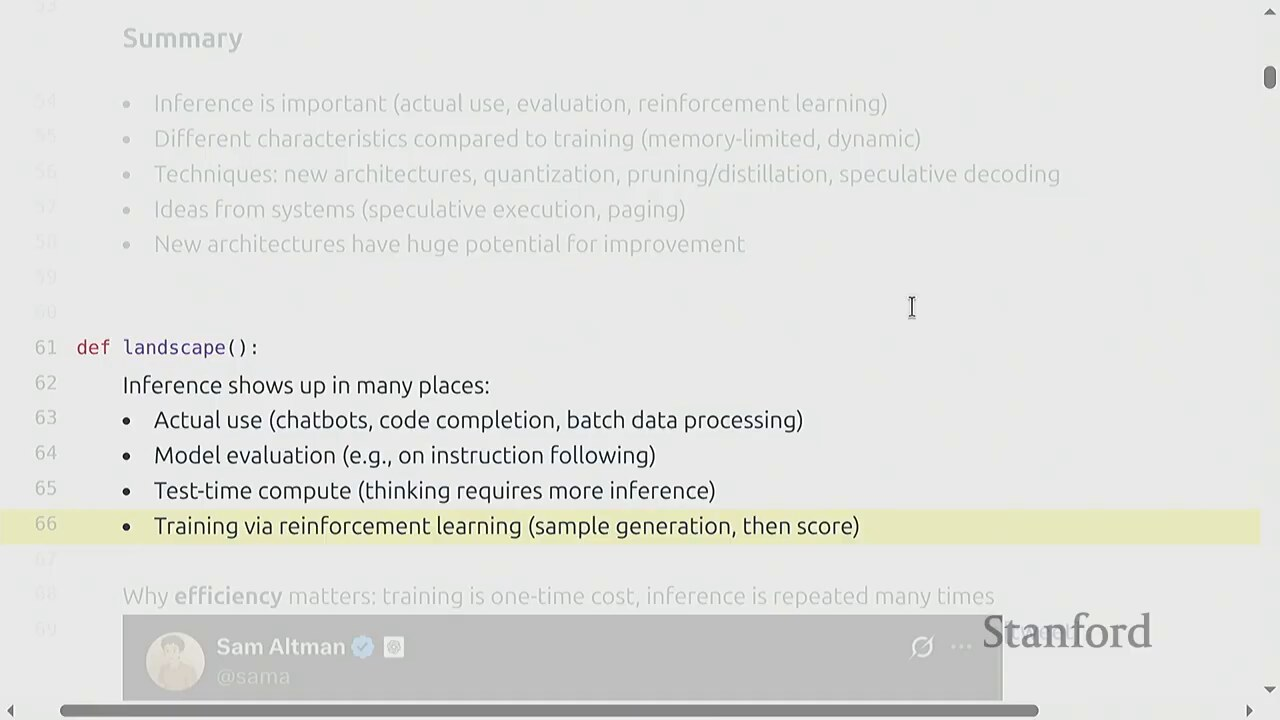
\includegraphics[width=\textwidth]{figures/fig_00_intro.jpg}
\caption{从训练到推理：serving 才是成本的大头\protect\footnotemark}
\end{figure}
\footnotetext{视频画面时间区间：00:01:45--00:02:15。}

\begin{importantbox}{为什么推理比训练更难优化}
训练是\textbf{一次大批次、长跑几周}，瓶颈集中、容易吃满硬件；推理是\textbf{高并发、变长请求、用户在等}，瓶颈分散且随负载变化。训练时可以容忍一点浪费，推理时每一毫秒都直接关系用户体验和运营成本。
\end{importantbox}

\subsection{推理性能的四个关键指标}

讲清楚优化目标之前，先要明确衡量指标。Percy 给出了四个核心量：

\begin{figure}[H]
\centering
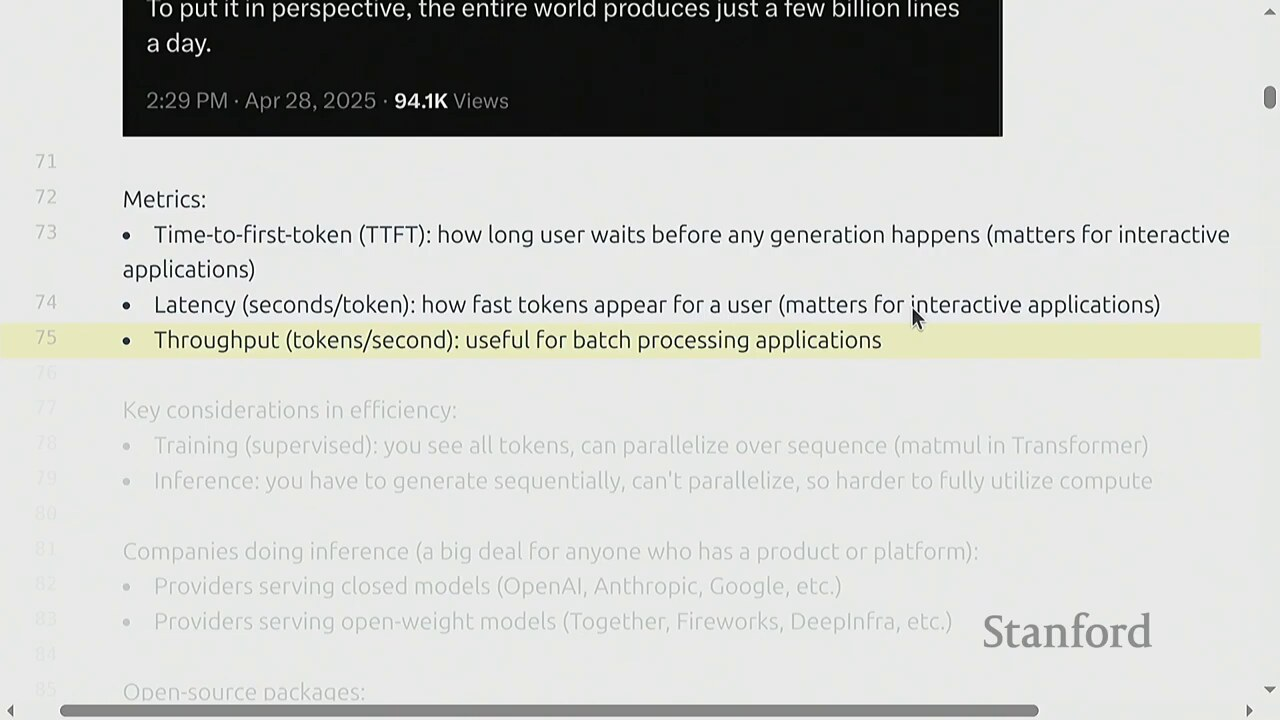
\includegraphics[width=\textwidth]{figures/fig_01_metrics.jpg}
\caption{推理服务的四大性能指标\protect\footnotemark}
\end{figure}
\footnotetext{视频画面时间区间：00:03:45--00:04:15。}

\begin{tabular}{p{3.5cm}p{2cm}p{8cm}}
\toprule
\textbf{指标} & \textbf{符号} & \textbf{含义} \\
\midrule
首 token 延迟 & TTFT & 用户发送请求到收到第一个 token 的时间，决定"是否卡顿" \\
单 token 延迟 & latency & 生成每个 token 的平均时间，决定"打字快慢" \\
吞吐 & throughput & 单位时间（每秒）整个系统生成的 token 总数 \\
成本 & cost & 每生成 100 万 token 需要多少美元 \\
\bottomrule
\end{tabular}

\begin{knowledgebox}{延迟与吞吐的对立统一}
延迟（每个用户感受到的速度）和吞吐（系统整体效率）常常是\textbf{此消彼长}的。批量把多个请求凑一起跑，能拉高吞吐，但单个请求可能要等凑批，延迟反而升高。本讲后半段的连续批处理（continuous batching）就是在这两者之间找最优解。
\end{knowledgebox}

\subsection{统一符号定义}

为了避免后面推导算术强度时符号混乱，先把全讲用到的记号固定下来：

\begin{figure}[H]
\centering
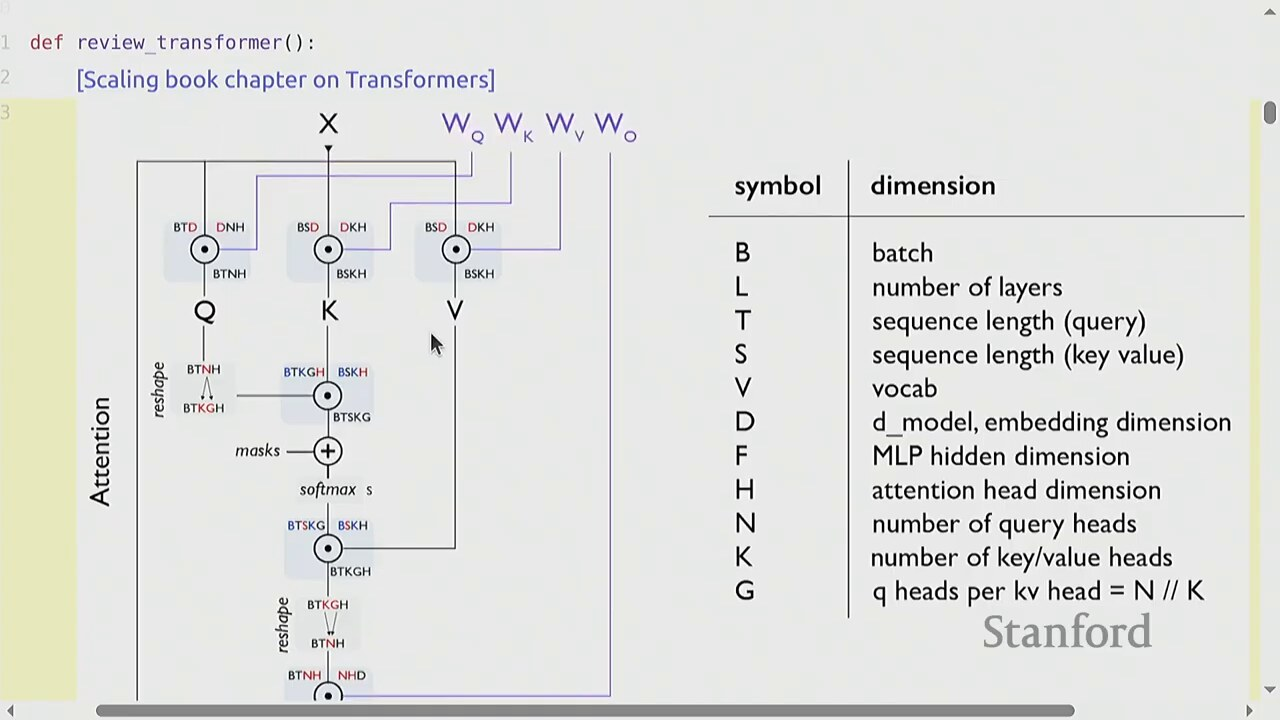
\includegraphics[width=\textwidth]{figures/fig_02_notation.jpg}
\caption{贯穿全讲的统一符号\protect\footnotemark}
\end{figure}
\footnotetext{视频画面时间区间：00:06:20--00:06:50。}

\begin{tabular}{p{2cm}p{12cm}}
\toprule
\textbf{符号} & \textbf{含义} \\
\midrule
$B$ & 批大小（batch size），同时处理的请求数 \\
$L$ & 序列长度，一个请求包含的 token 数 \\
$T$ & 解码阶段要生成的新 token 数 \\
$S$ & 上下文（prefill）长度，即 prompt 的 token 数 \\
$V$ & 词表大小（vocab size） \\
$D$ & 隐藏维度（hidden dimension），模型主干的特征宽度 \\
$H$ & 注意力头数 \\
\bottomrule
\end{tabular}

\section{算术强度：推理优化的统一框架}

本讲最重要的一个思维工具是\textbf{算术强度}（arithmetic intensity）。几乎所有推理优化技术，都可以用这一个概念串起来。

\subsection{矩阵乘法的 FLOPs 与字节}

先看最基本的操作——矩阵乘法。这是 Transformer 里最贵的算子。对一个形状为 $(B, D)$ 的输入乘以权重 $(D, D)$：

\begin{figure}[H]
\centering
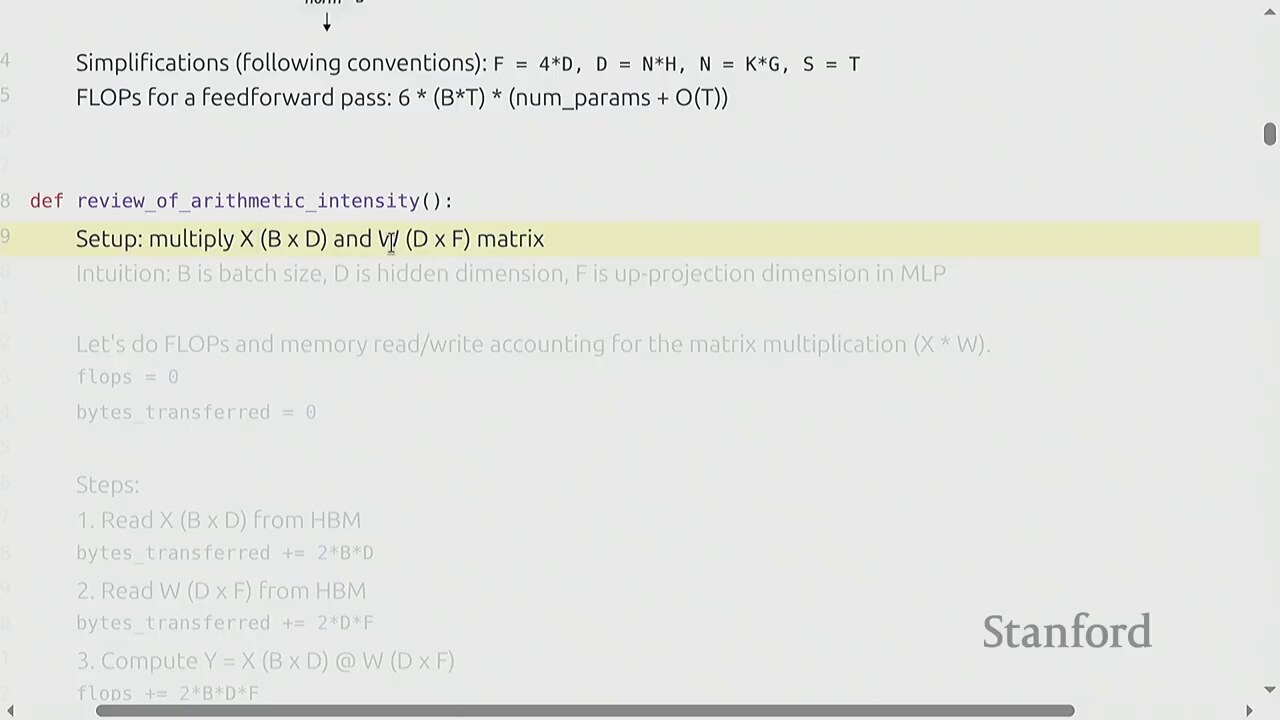
\includegraphics[width=\textwidth]{figures/fig_03_matmul.jpg}
\caption{矩阵乘法：算多少 FLOPs、读多少字节\protect\footnotemark}
\end{figure}
\footnotetext{视频画面时间区间：00:08:15--00:08:45。}

FLOPs 和数据搬运量分别是：

\[
\text{FLOPs} = 2 B D^2, \qquad \text{bytes} = 2 B D + 2 D^2
\]

\begin{itemize}
\item $2 B D^2$：输出矩阵每个元素需要 $2D$ 次乘加（乘和加各算一次），共 $B D$ 个输出元素
\item $2 B D$：读入激活矩阵的字节数（BF16 下每个元素 2 字节）
\item $2 D^2$：读入权重矩阵的字节数（权重每次都要重读）
\end{itemize}

\subsection{算术强度的定义}

\begin{importantbox}{算术强度的定义}
算术强度 $I$ 定义为\textbf{每读一个字节做了多少次浮点运算}：

\[
I = \frac{\text{FLOPs}}{\text{bytes}}
\]

它回答一个关键问题：这个算子到底是被\textbf{算力}卡住，还是被\textbf{带宽}卡住？
\end{importantbox}

对上面的矩阵乘，当 $B \gg 1$（大批量）时，权重 $2D^2$ 被很多请求摊薄，算术强度接近：

\[
I \approx \frac{2 B D^2}{2 D^2} = B
\]

而 $B = 1$（单请求）时，激活和权重同量级：

\[
I \approx \frac{2 D^2}{2 B D + 2 D^2} = \frac{D}{B + D} \xrightarrow{B=1} \approx 1
\]

\begin{warningbox}{关键直觉}
$B = 1$ 时算术强度约为 1——做一次乘加几乎只读一个字节。这意味着\textbf{单请求推理严重浪费算力}，瓶颈完全在显存带宽上。
\end{warningbox}

\subsection{H100 的 Roofline 阈值}

为什么算术强度重要？因为每块 GPU 都有一条\textbf{roofline}曲线——它既受峰值算力（FLOPS）限制，也受峰值带宽（bytes/s）限制。两条线交点对应的算术强度，叫做\textbf{转折点}：

\begin{figure}[H]
\centering
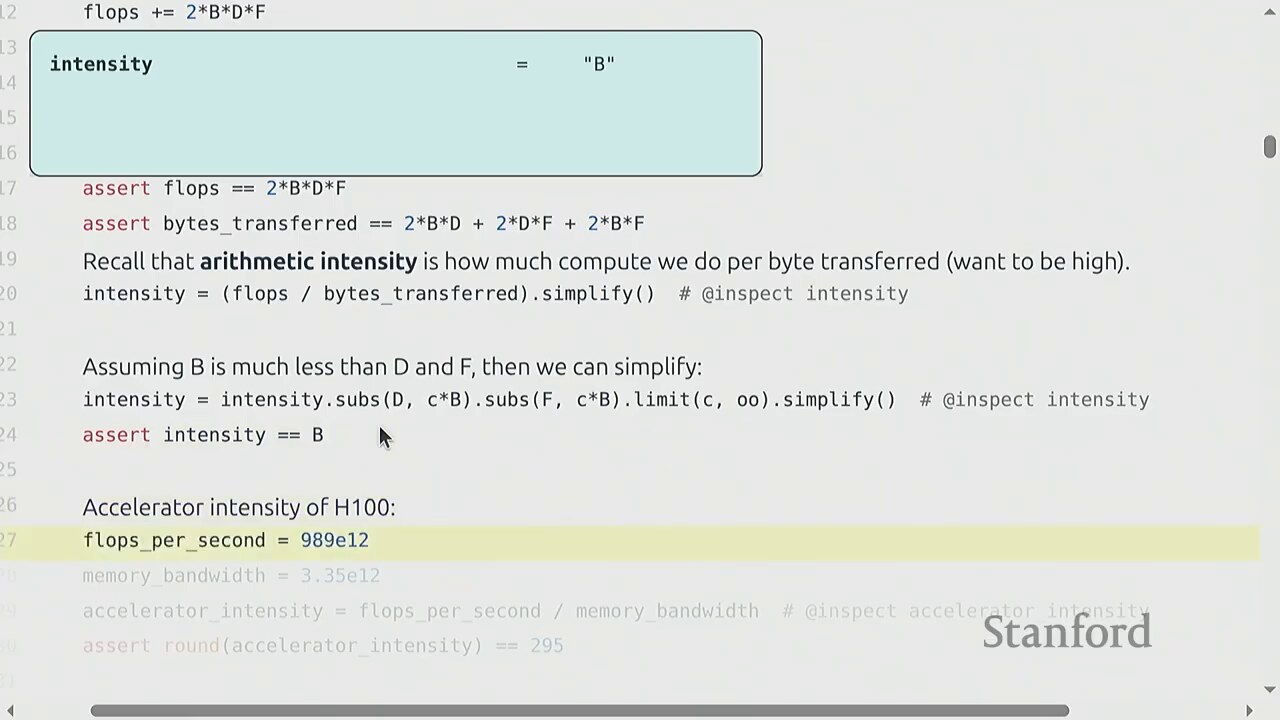
\includegraphics[width=\textwidth]{figures/fig_04_h100.jpg}
\caption{H100 的算力、带宽与算术强度阈值\protect\footnotemark}
\end{figure}
\footnotetext{视频画面时间区间：00:10:45--00:11:15。}

\[
I^* = \frac{\text{FLOPS}}{\text{bandwidth}}
\]

\begin{itemize}
\item $\text{FLOPS}$：GPU 每秒能做的浮点运算次数（H100 BF16 约 989 TFLOPS）
\item $\text{bandwidth}$：GPU 每秒能从显存读出的字节数（H100 HBM3 约 3.35 TB/s）
\item $I^*$：算术强度阈值，H100 上 $\approx 989/3.35 \approx 295$
\end{itemize}

\begin{knowledgebox}{Roofline 的判读规则}
若算子的 $I > I^*$，则\textbf{算力受限}（compute-bound）——加更多并发请求不会更快，因为已经把算力吃满了。若 $I < I^*$，则\textbf{带宽受限}（memory-bound）——光读权重就把时间耗光，算力闲置。H100 上这个阈值接近 300，是个非常高的门槛。
\end{knowledgebox}

\subsection{\texorpdfstring{$B=1$}{B=1}：典型的带宽受限场景}

把上面的数字代入单请求推理：

\begin{figure}[H]
\centering
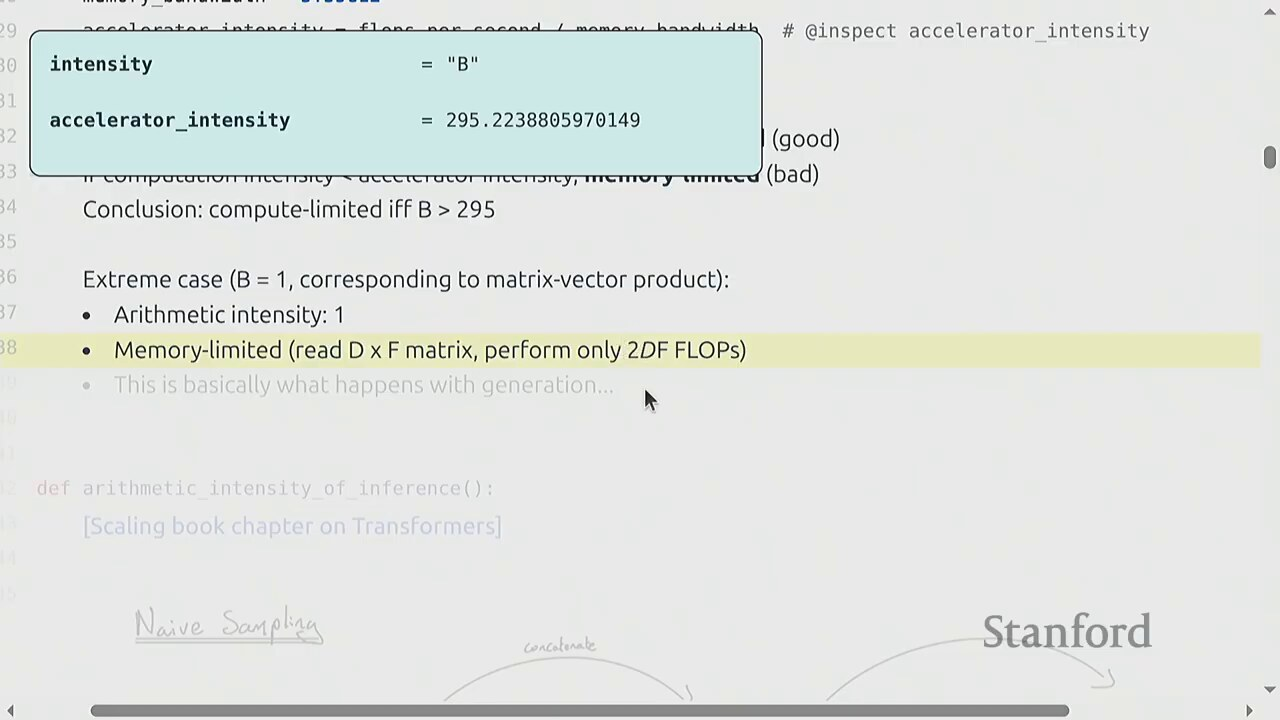
\includegraphics[width=\textwidth]{figures/fig_05_b1mem.jpg}
\caption{$B=1$ 时：算术强度约等于 1 远小于 300，纯带宽受限\protect\footnotemark}
\end{figure}
\footnotetext{视频画面时间区间：00:12:25--00:12:55。}

\begin{importantbox}{$B=1$ 的核心结论}
单请求解码时算术强度 $\approx 1$，远小于 H100 的阈值 300。意味着：你花大价钱买的 989 TFLOPS 算力，\textbf{实际只用了不到 1/300}。GPU 大部分时间在等显存把权重吐出来。这是所有推理优化技术的出发点。
\end{importantbox}

\section{KV Cache：避免重复计算}

\subsection{朴素实现的冗余}

如果不做任何缓存，自回归生成时每出一个新 token，都要重新算一遍前面所有 token 的注意力。这是巨大的浪费：

\begin{figure}[H]
\centering
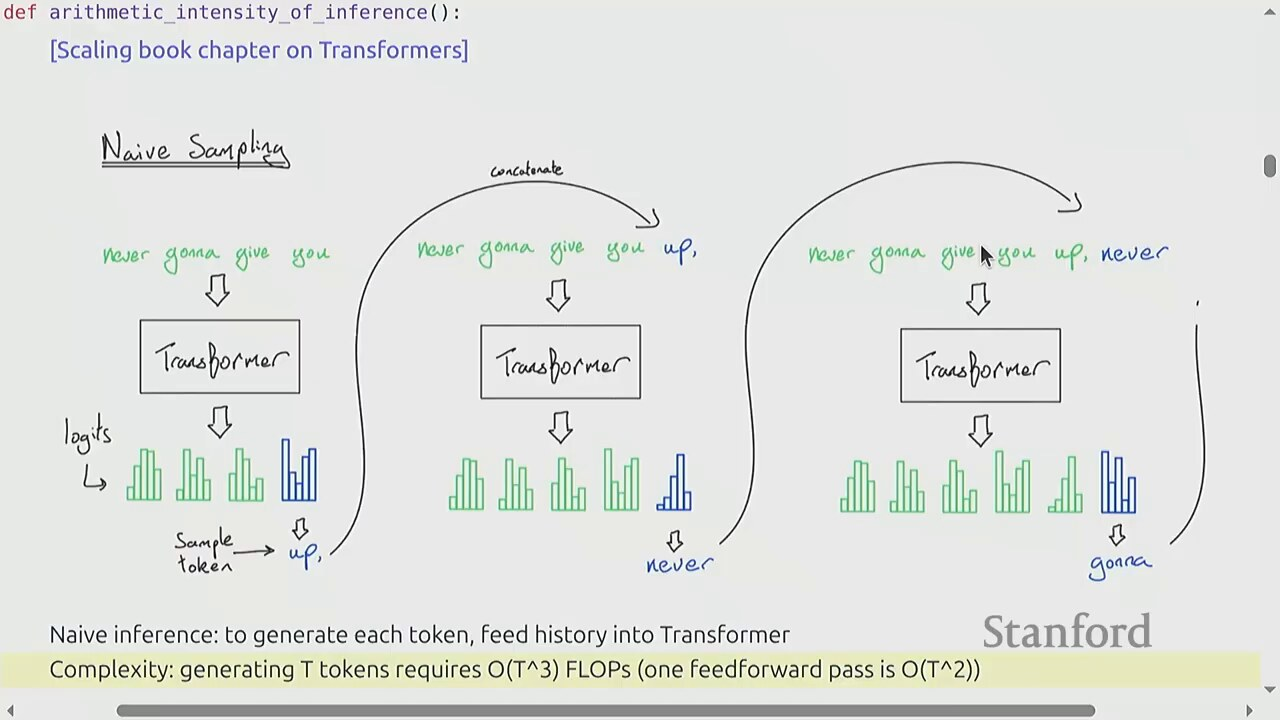
\includegraphics[width=\textwidth]{figures/fig_06_naive.jpg}
\caption{朴素实现：第 $t$ 步重算前 $t-1$ 步的所有注意力\protect\footnotemark}
\end{figure}
\footnotetext{视频画面时间区间：00:15:15--00:15:45。}

\begin{warningbox}{朴素的 $O(N^2)$ 之痛}
生成 $T$ 个 token，朴素实现的总开销正比于 $1 + 2 + \dots + T = O(T^2)$。每个 token 的延迟随已生成长度线性增长——这根本没法用于长对话。
\end{warningbox}

\subsection{KV Cache 的核心思想}

注意到注意力公式里，每个历史 token 只通过它的 $K$（键）和 $V$（值）参与计算，而且这两个量一旦算出来就\textbf{不变}——可以缓存下来复用：

\begin{figure}[H]
\centering
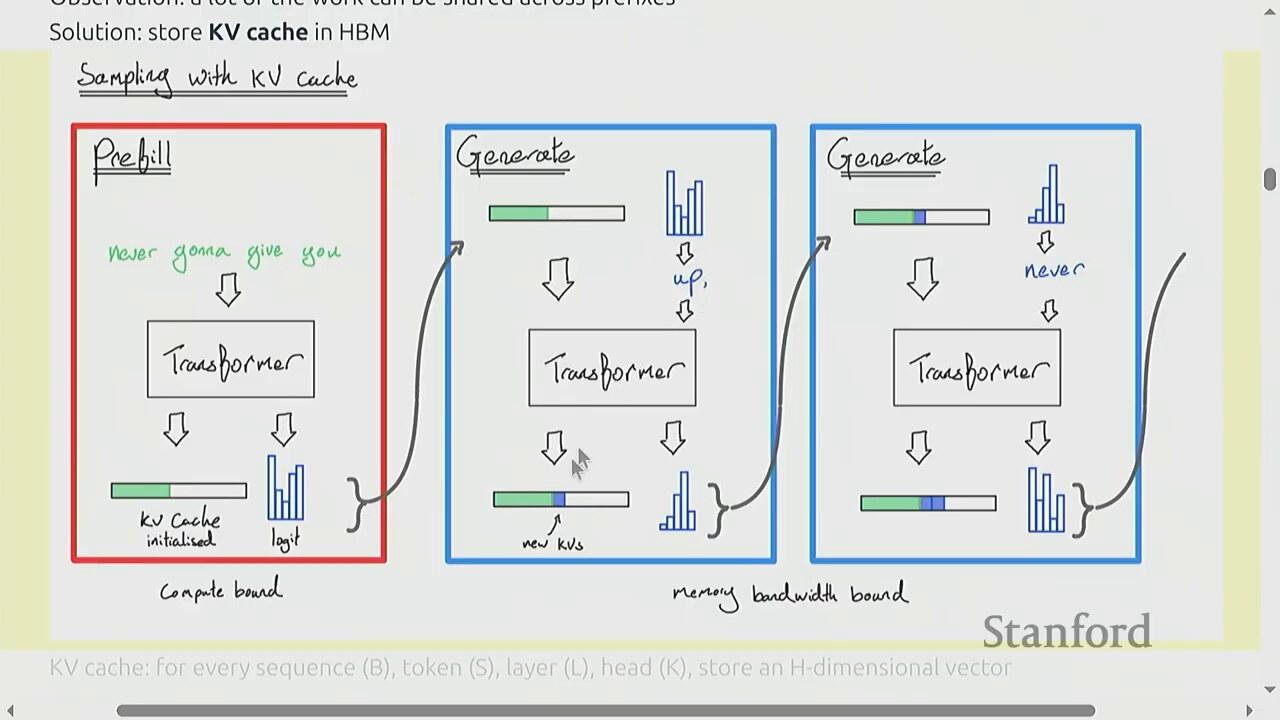
\includegraphics[width=\textwidth]{figures/fig_07_kvcache.jpg}
\caption{KV cache：缓存历史 token 的键值，下一步只算新 token 的注意力\protect\footnotemark}
\end{figure}
\footnotetext{视频画面时间区间：00:16:25--00:16:55。}

\begin{knowledgebox}{KV cache 的本质}
KV cache 用\textbf{空间换时间}：把每层每个头的 $(K, V)$ 存下来，避免每步重算。代价是显存占用随序列长度线性增长——这恰恰是后面"批量请求会 OOM"的根本原因。
\end{knowledgebox}

第 $t$ 步，只需读入新 token 算出它的 $q_t, k_t, v_t$，然后用 $q_t$ 与缓存里所有的 $K$ 做点积，再与 $V$ 加权求和。每步注意力是 $O(t)$ 而非 $O(t^2)$。

\subsection{推理的两个阶段：Prefill 与 Decode}

有了 KV cache，推理自然分成两个节奏完全不同的阶段：

\begin{figure}[H]
\centering
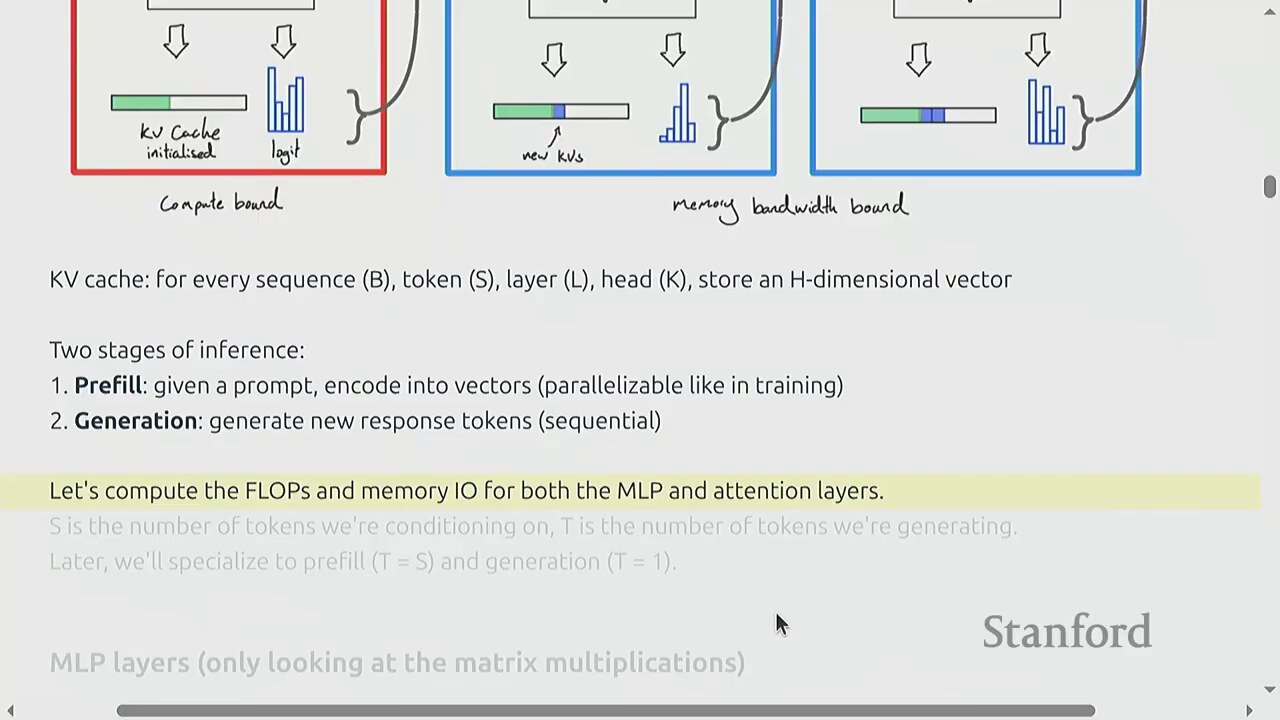
\includegraphics[width=\textwidth]{figures/fig_08_twostages.jpg}
\caption{Prefill（预填充）与 Decode（解码）两个阶段\protect\footnotemark}
\end{figure}
\footnotetext{视频画面时间区间：00:17:45--00:18:15。}

\begin{tabular}{p{2cm}p{6cm}p{6cm}}
\toprule
& \textbf{Prefill} & \textbf{Decode} \\
\midrule
做什么 & 一次性吃下整个 prompt，算出所有 token 的 KV 并缓存 & 逐个生成新 token，每步读 KV cache 算一个 token \\
批大小 & prompt 长度 $S$（通常几百到几千） & $B$ 个请求，每个只算 1 个 token \\
算术强度 & 高（$\approx S$） & 低（$\approx 1$） \\
瓶颈 & 算力（compute-bound） & 带宽（memory-bound） \\
\bottomrule
\end{tabular}

\begin{figure}[H]
\centering
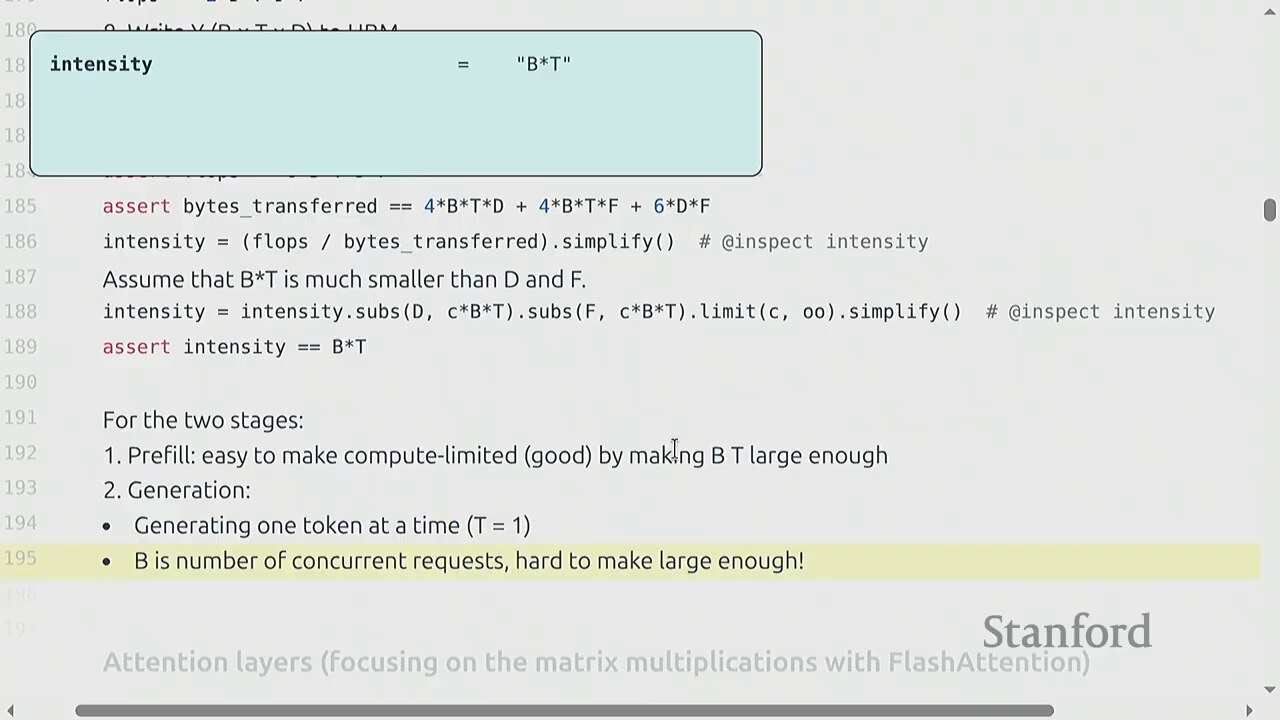
\includegraphics[width=\textwidth]{figures/fig_09_prefill.jpg}
\caption{Prefill 阶段：大批量矩阵乘，算术强度 $\approx S$\protect\footnotemark}
\end{figure}
\footnotetext{视频画面时间区间：00:21:15--00:21:45。}

\begin{importantbox}{Prefill 是算力受限}
Prefill 把 prompt 当作一个 $B=S$ 的大批次做矩阵乘，算术强度 $\approx S$（几百到几千），远超 H100 阈值 300。这一阶段把算力吃满，是\textbf{compute-bound}。优化方向是张量并行、更好的 kernel。
\end{importantbox}

\section{注意力的算术强度推导}

Percy 接下来用一个漂亮的小推导，回答了一个看似细节、实则关键的问题：解码阶段的\textbf{注意力本身}，算术强度到底是多少？

\subsection{Decode 阶段的注意力：\texorpdfstring{$\sim ST/(S+T)$}{~ST/(S+T)}}

\begin{figure}[H]
\centering
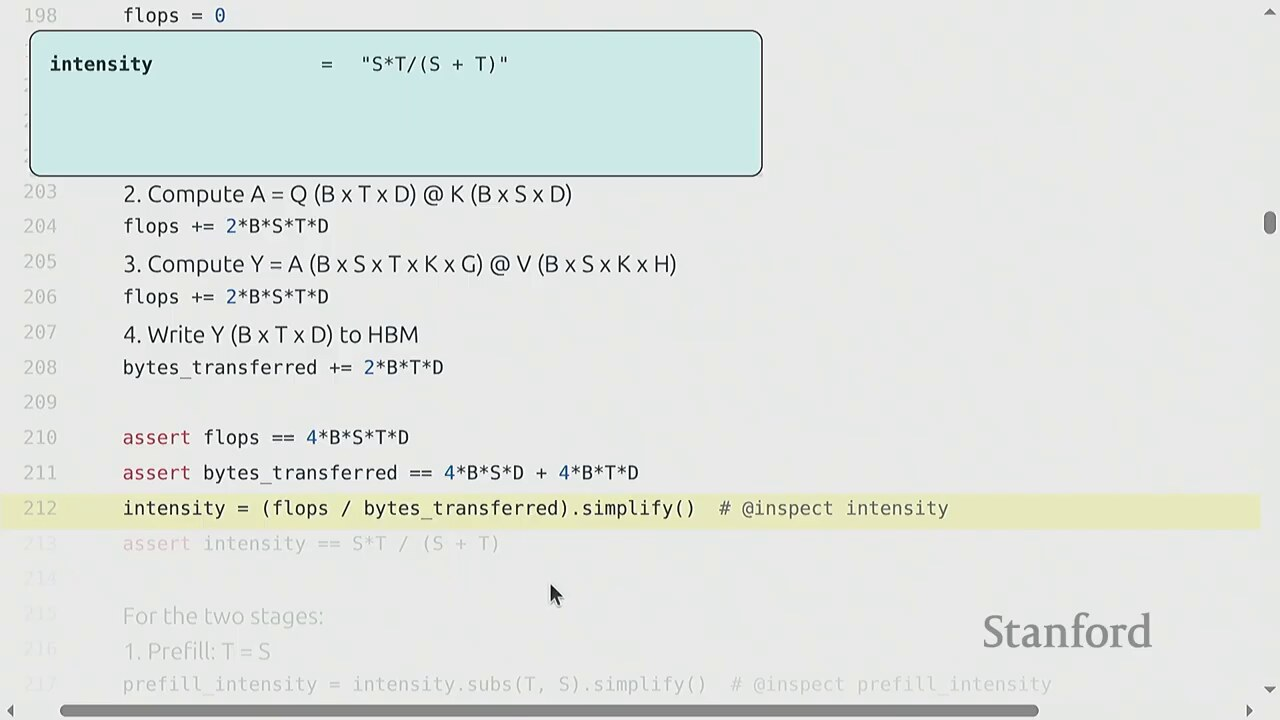
\includegraphics[width=\textwidth]{figures/fig_10_attnst.jpg}
\caption{解码注意力的算术强度 $\sim ST/(S+T)$\protect\footnotemark}
\end{figure}
\footnotetext{视频画面时间区间：00:23:55--00:24:25。}

设上下文长度 $S$、生成长度 $T$。每步解码，注意力的 FLOPs 来自 $q$ 与所有 $K$ 的点积，以及 softmax 后与 $V$ 的加权求和：

\[
\text{FLOPs}_{\text{attn}} \sim B \cdot (S + T) \cdot D, \qquad \text{bytes}_{\text{attn}} \sim B \cdot (S + T) \cdot D
\]

\begin{itemize}
\item $B \cdot (S+T) \cdot D$：要读的 KV cache 字节数（每个历史 token 的 K 和 V）
\item 注意力的 FLOPs 与读的字节\textbf{同量级}，因为每个 KV 元素只参与 $O(1)$ 次乘加
\end{itemize}

把整个生成过程平均下来，每个 token 的有效算术强度约为：

\[
I_{\text{attn}} \sim \frac{S T}{S + T}
\]

\subsection{当 \texorpdfstring{$T \gg S$}{T >> S}：算术强度趋于 1}

当生成很长（$T \gg S$，即多轮长对话），分母里 $S$ 可忽略：

\begin{figure}[H]
\centering
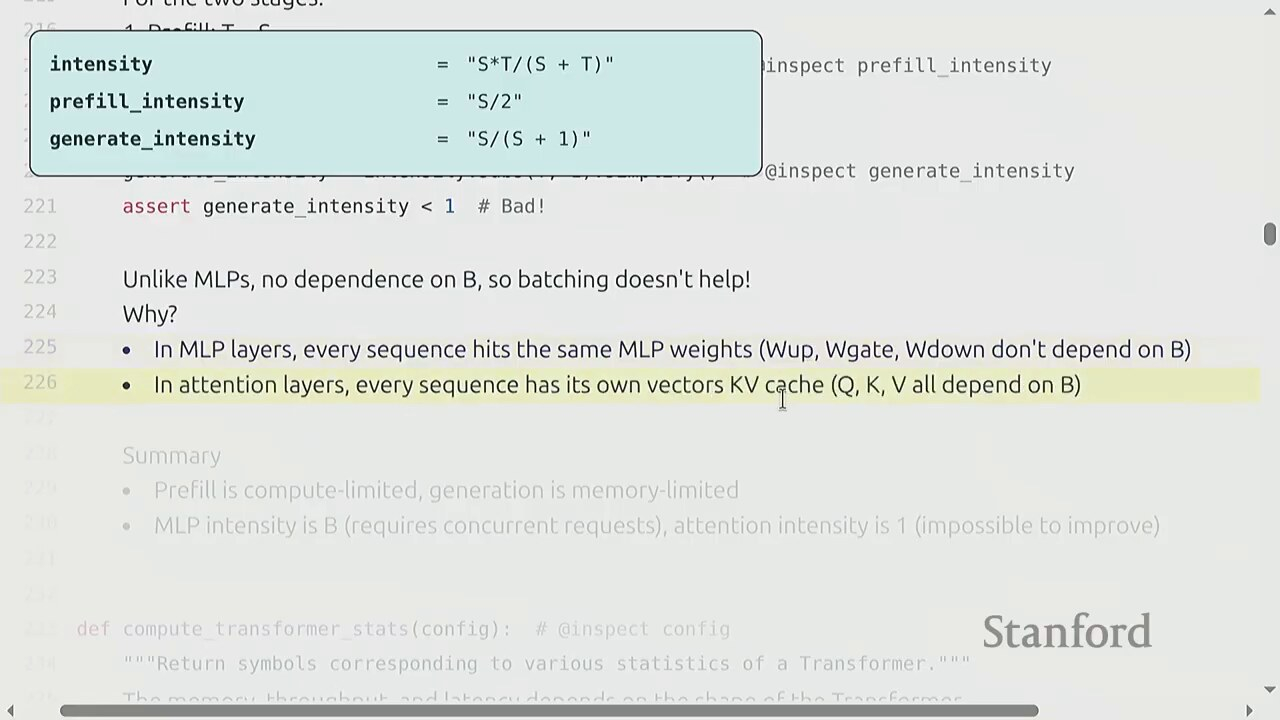
\includegraphics[width=\textwidth]{figures/fig_11_attn1.jpg}
\caption{$T \gg S$ 时：解码注意力强度 $\to S$（仍远低于阈值）\protect\footnotemark}
\end{figure}
\footnotetext{视频画面时间区间：00:25:35--00:26:05。}

\[
I_{\text{attn}} \xrightarrow{T \gg S} S
\]

\begin{warningbox}{注意力的致命弱点}
即便考虑上下文长度 $S$，注意力的算术强度也只有 $S$ 量级（几千），而每个 token 的\textbf{读写量}（KV cache 体积）随序列长度线性膨胀。\textbf{注意力层的瓶颈永远是带宽}，而且越长的上下文越严重。这就是为什么后面所有架构改造（GQA、MLA、SSM）都在攻击 KV cache 的体积。
\end{warningbox}

\begin{importantbox}{MLP 与注意力的对比}
对比之下，MLP 层（前馈网络）每个 token 要乘两个大权重矩阵，算术强度 $\approx B$——所以\textbf{加大批量}能直接让 MLP 变得算力受限、提高 GPU 利用率。但注意力的强度\textbf{与 $B$ 无关}，加批量救不了它。这是本讲最重要的不对称性。
\end{importantbox}

\section{Llama2 手算：把公式落到具体数字}

理论讲完，Percy 用 Llama2 的真实配置做了一次"餐巾纸算术"（napkin math），让所有公式落地：

\begin{figure}[H]
\centering
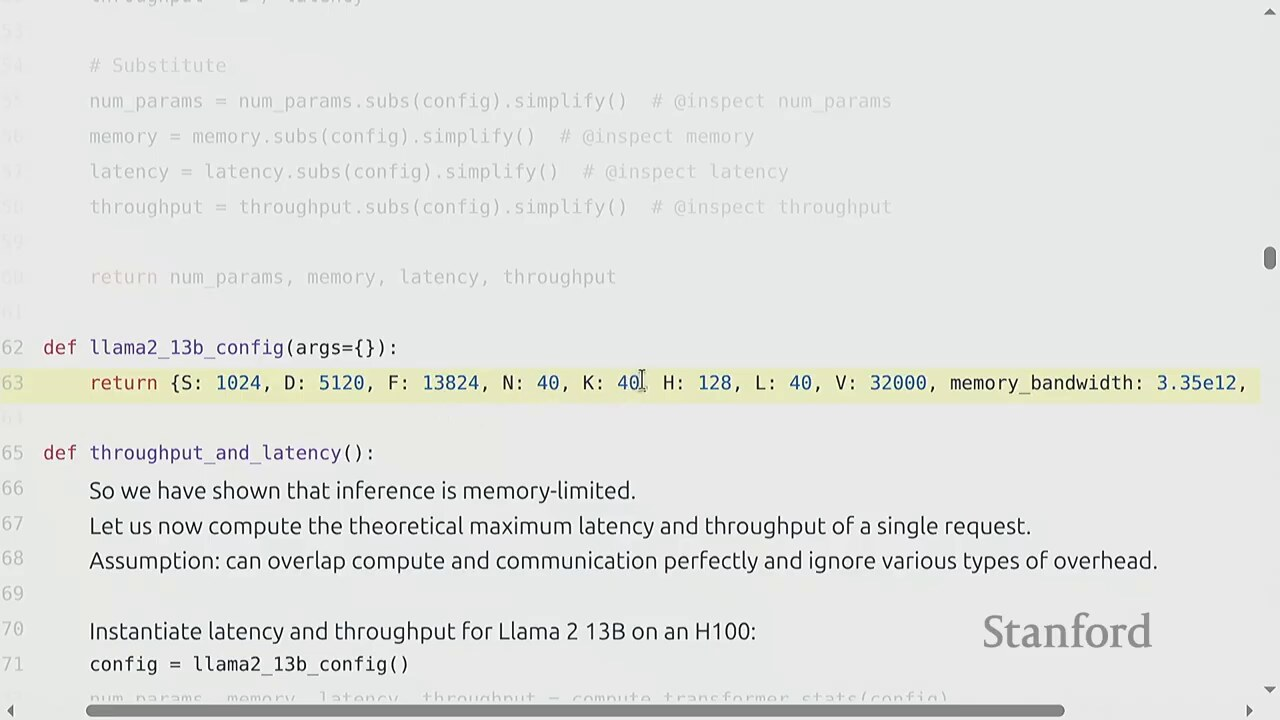
\includegraphics[width=\textwidth]{figures/fig_12_llama2.jpg}
\caption{Llama2 配置与单卡推理性能估算\protect\footnotemark}
\end{figure}
\footnotetext{视频画面时间区间：00:28:45--00:29:15。}

Llama2-7B 的关键参数：层数 $L = 32$，隐藏维度 $D = 4096$，头数 $H = 32$，每个权重大约 70 亿参数。单次前向（生成 1 个 token）需要：

\[
\text{FLOPs}_{\text{token}} \approx 2 \cdot N_{\text{params}} = 2 \times 7\text{B} = 14 \text{ GFLOPs}
\]

而要把权重全读一遍（BF16）：

\[
\text{bytes}_{\text{token}} \approx 2 \cdot N_{\text{params}} = 14 \text{ GB}
\]

\begin{itemize}
\item $N_{\text{params}}$：模型参数量（Llama2-7B 约 70 亿）
\item $2 \cdot N_{\text{params}}$：每个 token 要算的 FLOPs（乘加各算一次），BF16 下也是要读的字节数
\end{itemize}

\begin{practicebox}{单 token 时间的下界}
单请求解码时算术强度 $\approx 1$，所以每秒能生成的 token 数被带宽卡死：

\[
\text{tokens/s} \approx \frac{\text{bandwidth}}{\text{bytes}_{\text{token}}} = \frac{3.35 \text{ TB/s}}{14 \text{ GB}} \approx 240 \text{ tokens/s}
\]

这是\textbf{理论下界}——单卡单请求，Llama2-7B 最多每秒吐约 240 个 token（实际因 kernel 开销会更低）。
\end{practicebox}

\subsection{批量：把吞吐拉上去}

单请求只用了带宽、算力闲置。把多个请求凑成一拨跑，权重只读一次、服务多个请求，算术强度就上去了：

\begin{figure}[H]
\centering
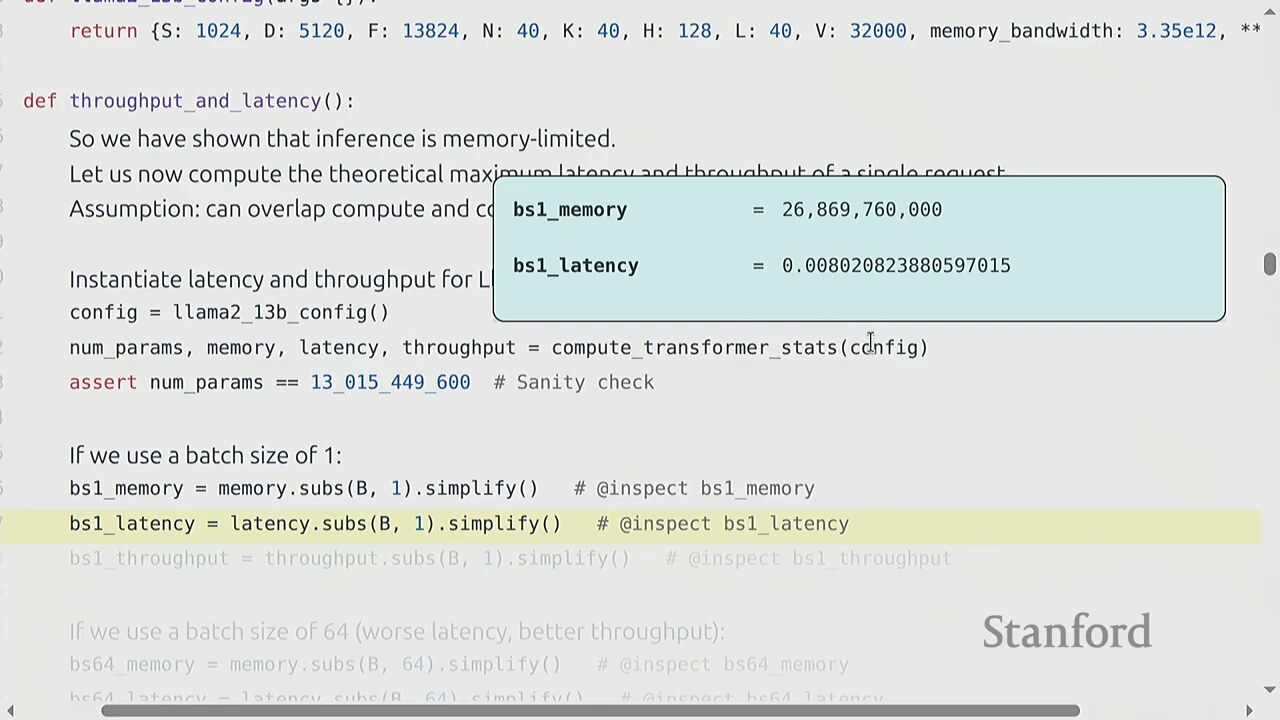
\includegraphics[width=\textwidth]{figures/fig_13_batch.jpg}
\caption{加大批量：吞吐上升、单 token 延迟不变（带宽足够宽）\protect\footnotemark}
\end{figure}
\footnotetext{视频画面时间区间：00:32:15--00:32:45。}

\begin{importantbox}{批量的甜区}
在带宽受限区，加大批量 $B$ 能让吞吐\textbf{线性增长}（因为算力还没饱和），同时\textbf{单 token 延迟几乎不变}（带宽够宽，多读点 KV 不碍事）。这是 serving 的"免费午餐"——直到两个限制出现：（1）KV cache 把显存撑爆；（2）算力饱和，开始互相挤。
\end{importantbox}

\subsection{\texorpdfstring{$B=256$}{B=256}：KV cache 把显存撑爆}

\begin{figure}[H]
\centering
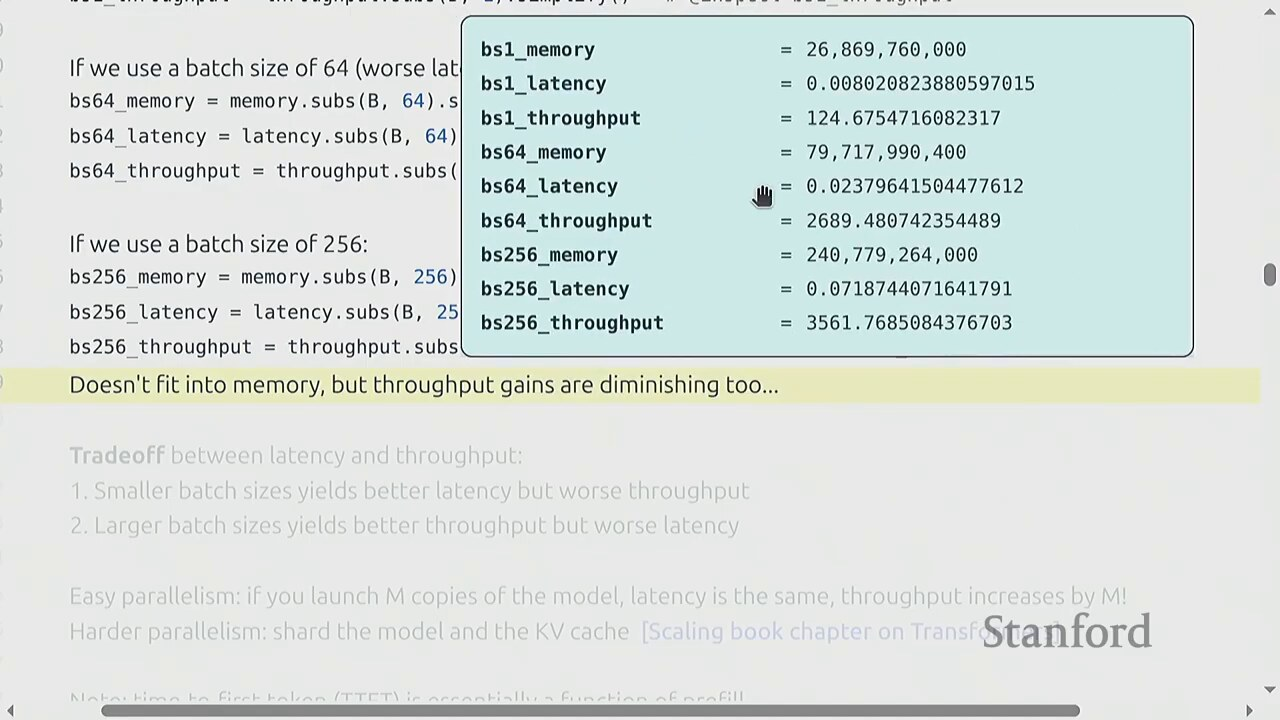
\includegraphics[width=\textwidth]{figures/fig_14_oomb256.jpg}
\caption{$B=256$ 时：KV cache 占满显存，OOM\protect\footnotemark}
\end{figure}
\footnotetext{视频画面时间区间：00:33:35--00:34:05。}

KV cache 的显存占用为：

\[
\text{KV memory} = 2 \cdot L \cdot H \cdot D_{\text{head}} \cdot (S + T) \cdot B \cdot 2 \text{ bytes}
\]

\begin{itemize}
\item $2$：K 和 V 两个张量
\item $L$：层数，$H$：头数，$D_{\text{head}} = D/H$：每头维度
\item $(S+T)$：每条请求的序列总长
\item $B$：批大小，最后乘 2 bytes 是 BF16
\end{itemize}

Llama2-7B 上，$B = 256$、$S = T = 2048$ 时，KV cache 就要吃掉几十 GB，远超单卡显存。\textbf{显存成了批量的天花板}。

\subsection{复制与张量并行：跨卡扩展}

单卡装不下怎么办？两条路：

\begin{figure}[H]
\centering
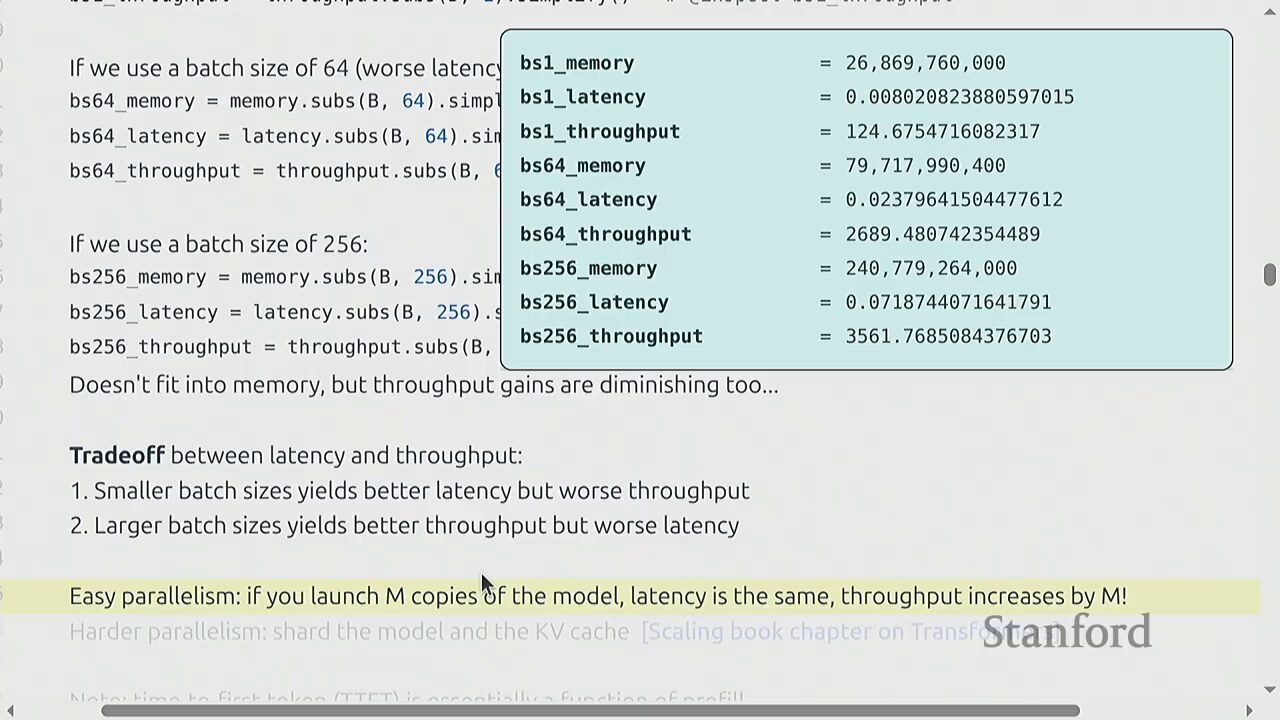
\includegraphics[width=\textwidth]{figures/fig_15_parallel.jpg}
\caption{复制（多份模型接不同请求）vs 张量并行（一切模型分到多卡）\protect\footnotemark}
\end{figure}
\footnotetext{视频画面时间区间：00:34:25--00:34:55。}

\begin{tabular}{p{3cm}p{6cm}p{6cm}}
\toprule
& \textbf{复制（replication）} & \textbf{张量并行（TP）} \\
\midrule
做法 & 同一模型拷贝几份，每份独立接不同请求 & 一个模型切成几块，每块放一张卡，请求同时跑 \\
适用 & 模型小、单卡装得下 & 模型大、单卡装不下 \\
吞吐 & 线性扩展（最理想） & 受通信开销影响 \\
延迟 & 不变 & 略升（要跨卡同步） \\
\bottomrule
\end{tabular}

\begin{knowledgebox}{复制的隐藏代价}
复制虽然吞吐线性扩展，但每份拷贝都要存完整的权重——显存利用率低。当请求量小时，多份拷贝可能各跑各的低批量，反而比一份统一跑大批量更亏。这就是为什么有"selective batching"——只在能凑批量时合并，否则拆开。
\end{knowledgebox}

\section{改造架构：降低推理的固有成本}

接下来 Percy 转向一个更深层的问题：上面的分析都假设了\textbf{标准 Transformer 架构}。如果改架构，能不能从根上把推理成本降下来？

\begin{figure}[H]
\centering
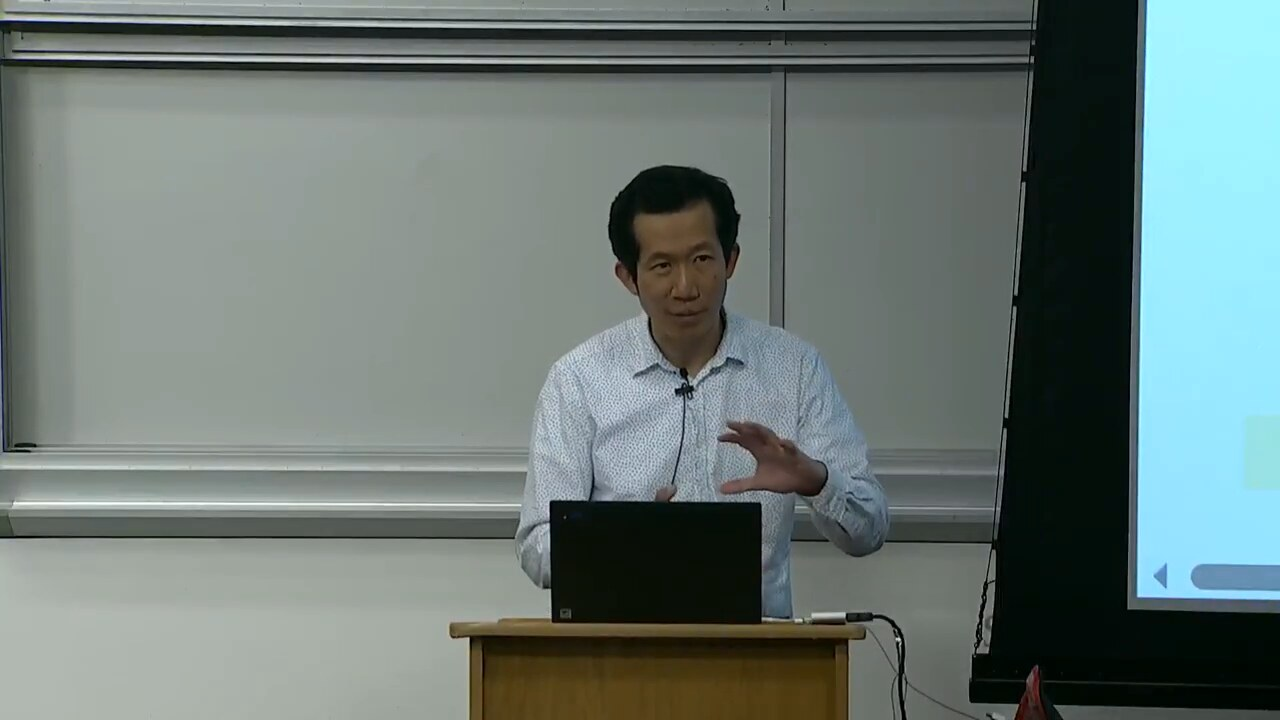
\includegraphics[width=\textwidth]{figures/fig_16_overviewarch.jpg}
\caption{降低推理成本的架构改造路线图\protect\footnotemark}
\end{figure}
\footnotetext{视频画面时间区间：00:36:45--00:37:15。}

\subsection{标准 MHA：KV cache 的代价}

先看标准的\textbf{多头注意力}（Multi-Head Attention）。每个头 $h$ 都有自己独立的 $K_h, V_h$：

\begin{figure}[H]
\centering
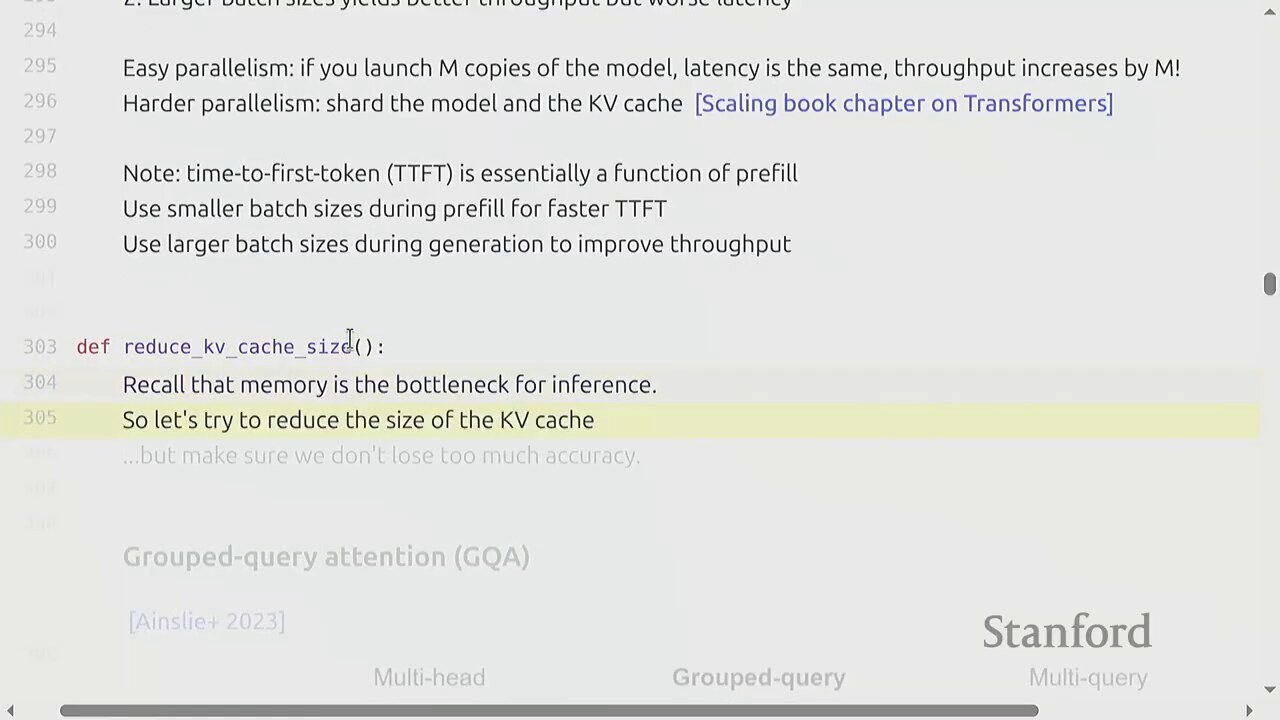
\includegraphics[width=\textwidth]{figures/fig_17_mha.jpg}
\caption{标准 MHA：$H$ 个头各存自己的 KV\protect\footnotemark}
\end{figure}
\footnotetext{视频画面时间区间：00:38:45--00:39:15。}

KV cache 总体积正比于 $H \cdot D_{\text{head}}$。头数越多，KV cache 越胖，带宽压力越大。

\subsection{MQA：所有头共享一组 KV}

\textbf{Multi-Query Attention}（MQA）做了一个激进的简化：所有查询头共享\textbf{同一组} $K, V$：

\begin{figure}[H]
\centering
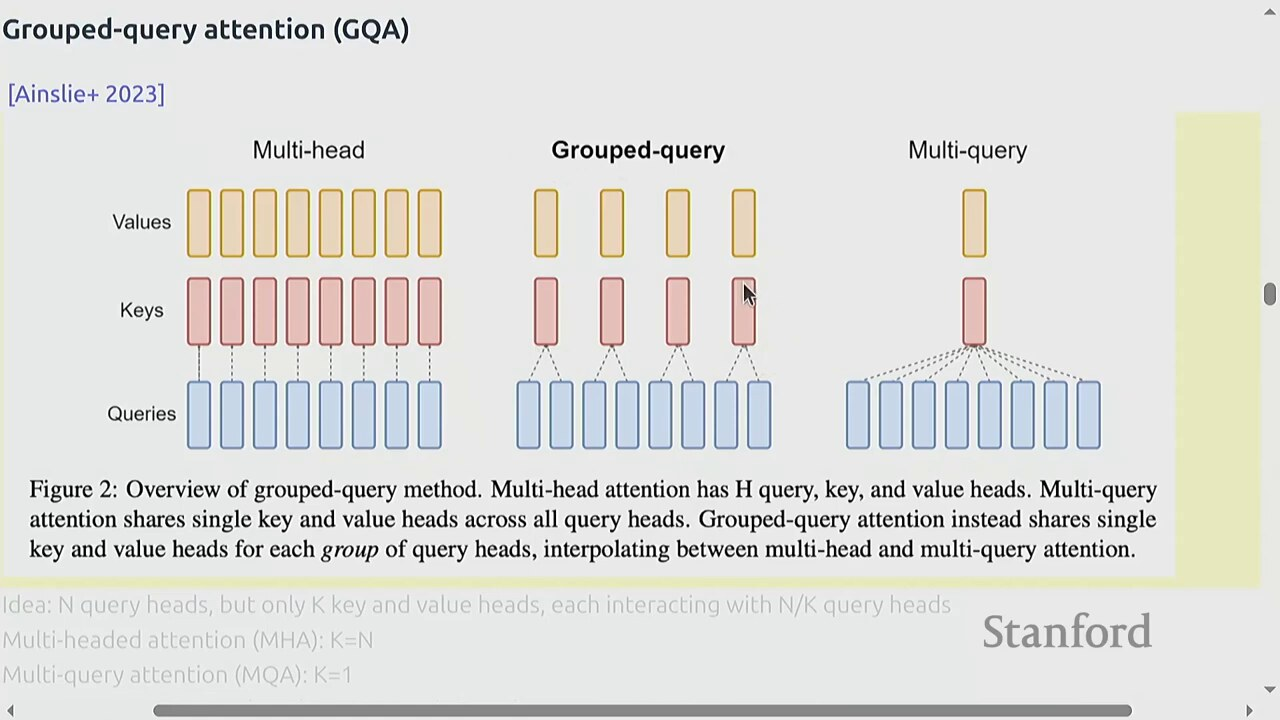
\includegraphics[width=\textwidth]{figures/fig_18_mqa.jpg}
\caption{MQA：所有查询头共享一组 KV，体积降至 $1/H$\protect\footnotemark}
\end{figure}
\footnotetext{视频画面时间区间：00:40:15--00:40:45。}

\begin{importantbox}{MQA 的取舍}
KV cache 体积直接降到 $1/H$（如 $H=32$ 就是 32 倍节省），带宽和显存压力大幅下降。代价是：所有查询头看的是同一份 KV，表达能力下降，模型质量略降。在\textbf{推理速度}远比"一点点精度"重要的场景，这笔交易非常划算。
\end{importantbox}

\subsection{GQA：折中方案}

Llama2-70B 等采用 \textbf{Grouped-Query Attention}（GQA），在 MHA 和 MQA 之间取折中：把 $H$ 个查询头分成 $G$ 组，每组共享一组 KV：

\begin{figure}[H]
\centering
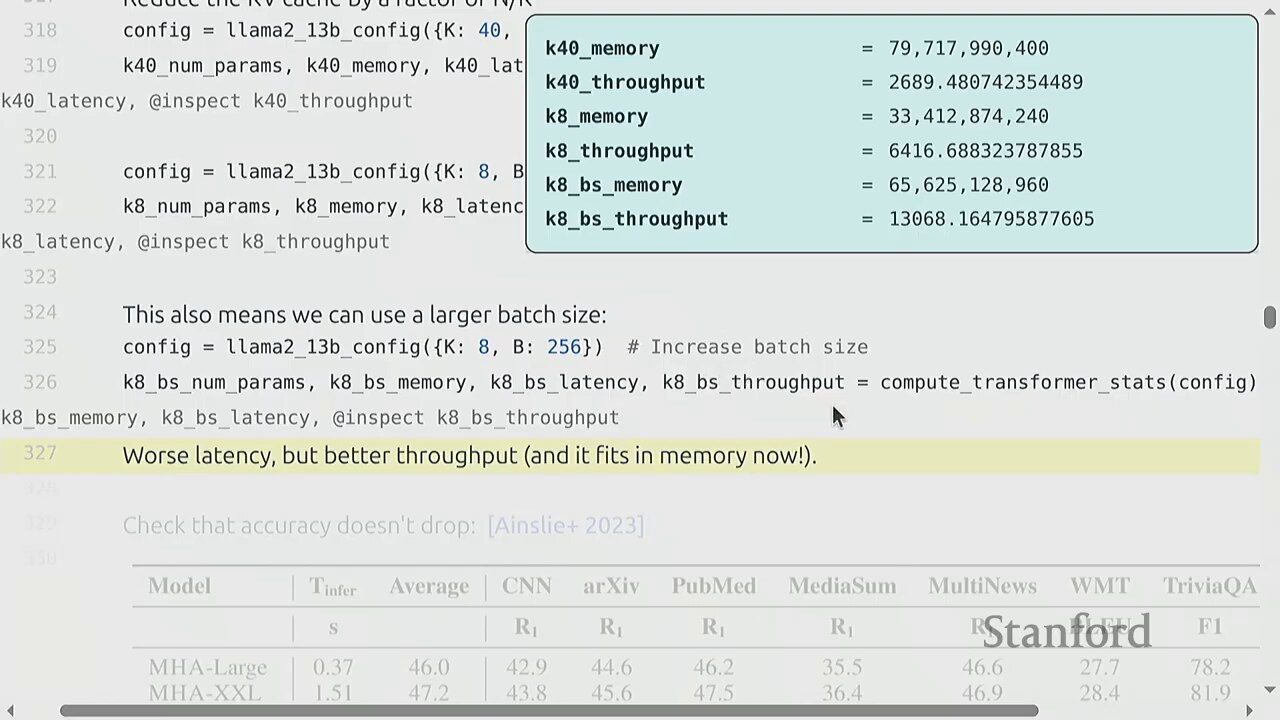
\includegraphics[width=\textwidth]{figures/fig_19_gqa.jpg}
\caption{GQA：$H$ 个查询头分 $G$ 组，组内共享 KV\protect\footnotemark}
\end{figure}
\footnotetext{视频画面时间区间：00:42:15--00:42:45。}

\begin{itemize}
\item $G = H$：退化为标准 MHA（每组只有一个头，各自独立）
\item $G = 1$：退化为 MQA（所有头一组）
\item $1 < G < H$：KV cache 体积是 MHA 的 $G/H$，质量损失比 MQA 小
\end{itemize}

\begin{knowledgebox}{为什么 GQA 是主流}
GQA 提供了一个平滑旋钮——在显存/带宽节省和模型质量之间连续调节。Llama2-70B 用 $G=8$（$H=64$），KV cache 省 8 倍但质量几乎不损。这种"几乎免费"的优化让 GQA 成了新一代大模型的标配。
\end{knowledgebox}

\subsection{MLA：DeepSeek 的低秩压缩}

\textbf{Multi-head Latent Attention}（MLA，DeepSeek 提出）更进一步：把 KV 压缩到一个\textbf{低秩潜在向量}，只在需要时才展开成完整的 K、V：

\begin{figure}[H]
\centering
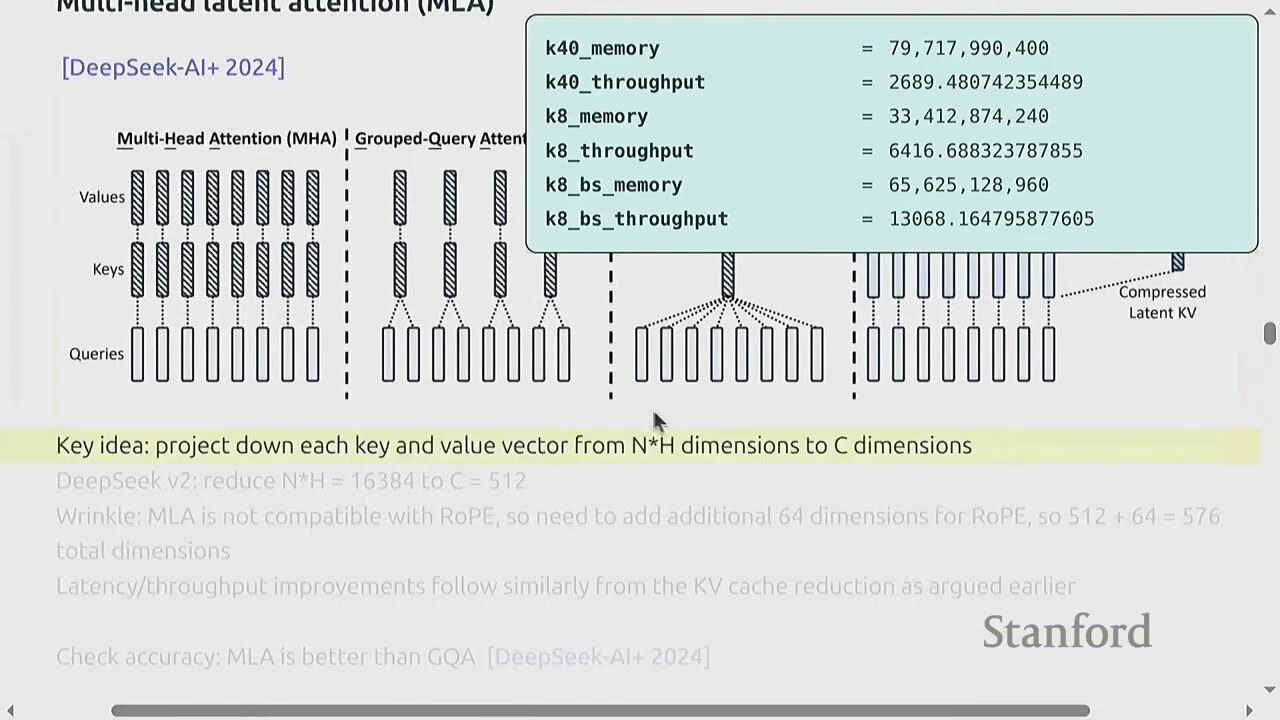
\includegraphics[width=\textwidth]{figures/fig_20_mla.jpg}
\caption{MLA（DeepSeek）：KV 先压到低秩潜在向量 $c$，再投影展开\protect\footnotemark}
\end{figure}
\footnotetext{视频画面时间区间：00:44:15--00:44:45。}

\[
K = W_K \, c, \qquad V = W_V \, c, \qquad c = W_c \, x
\]

\begin{itemize}
\item $x$：输入隐藏状态（高维 $D$）
\item $c$：压缩后的潜在向量（低维 $d_c \ll D \cdot H$）
\item $W_K, W_V$：把潜在向量投影回完整 K、V 的矩阵
\end{itemize}

\begin{importantbox}{MLA 的精妙}
MLA 只缓存\textbf{压缩向量 $c$}，而不是完整的 K、V。需要时再用 $W_K, W_V$ 投影出来。这让 KV cache 体积再降一个数量级，同时保留了多头的表达能力。代价是额外的投影计算，但在带宽受限的解码阶段，省下的带宽远比多算的 FLOPs 划算。
\end{importantbox}

\subsection{局部注意力与跨层共享}

除了改 KV 的组织方式，还可以\textbf{减少每个 token 需要存的 KV 数量}：

\begin{figure}[H]
\centering
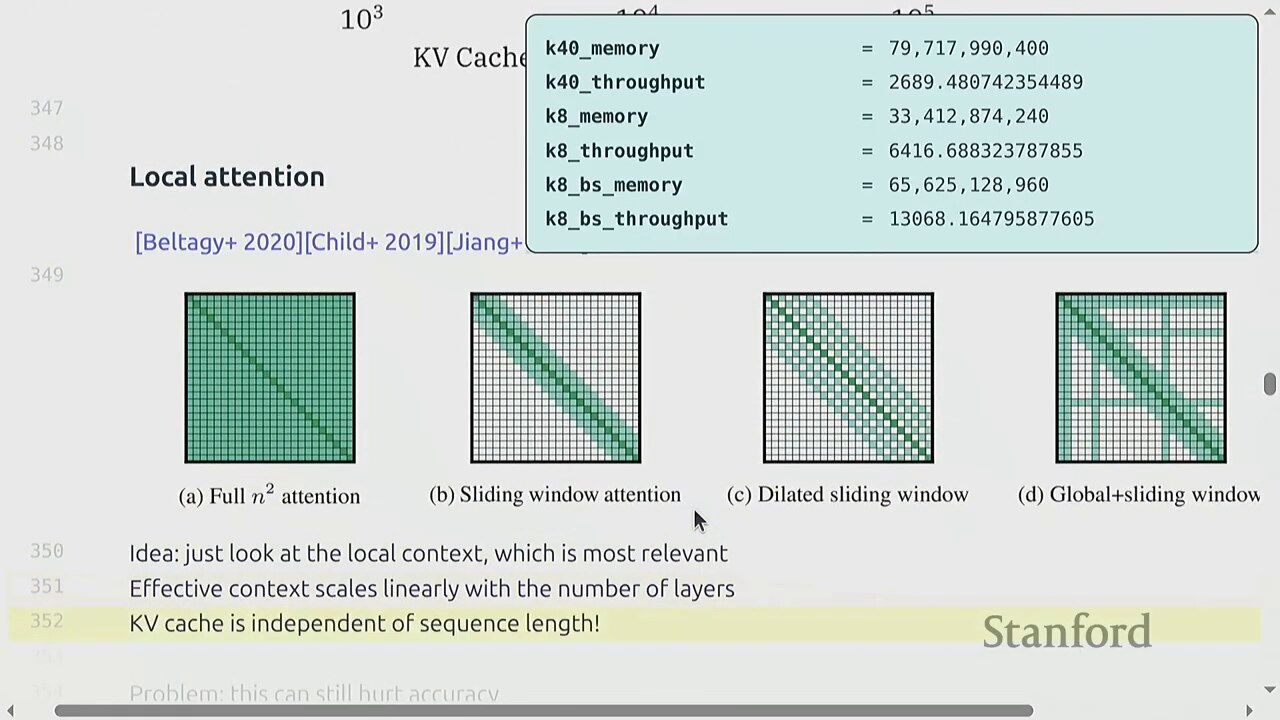
\includegraphics[width=\textwidth]{figures/fig_21_local.jpg}
\caption{局部/滑动窗口注意力 + CLA 跨层共享 KV\protect\footnotemark}
\end{figure}
\footnotetext{视频画面时间区间：00:48:45--00:49:15。}

\begin{tabular}{p{4cm}p{10cm}}
\toprule
\textbf{技术} & \textbf{做法与代价} \\
\midrule
滑动窗口注意力 & 每个 token 只看最近 $w$ 个 token，KV cache 大小恒定 $O(w)$。代价：丢失远距离依赖 \\
跨层注意力（CLA） & 相邻层共享同一份 KV，少算几组 K、V。代价：层间耦合，可能影响表达力 \\
\bottomrule
\end{tabular}

\subsection{状态空间模型（SSM / Mamba）}

更激进的思路：\textbf{换掉注意力本身}。状态空间模型用一个固定大小的隐状态 $h_t$ 替代变长的 KV cache：

\begin{figure}[H]
\centering
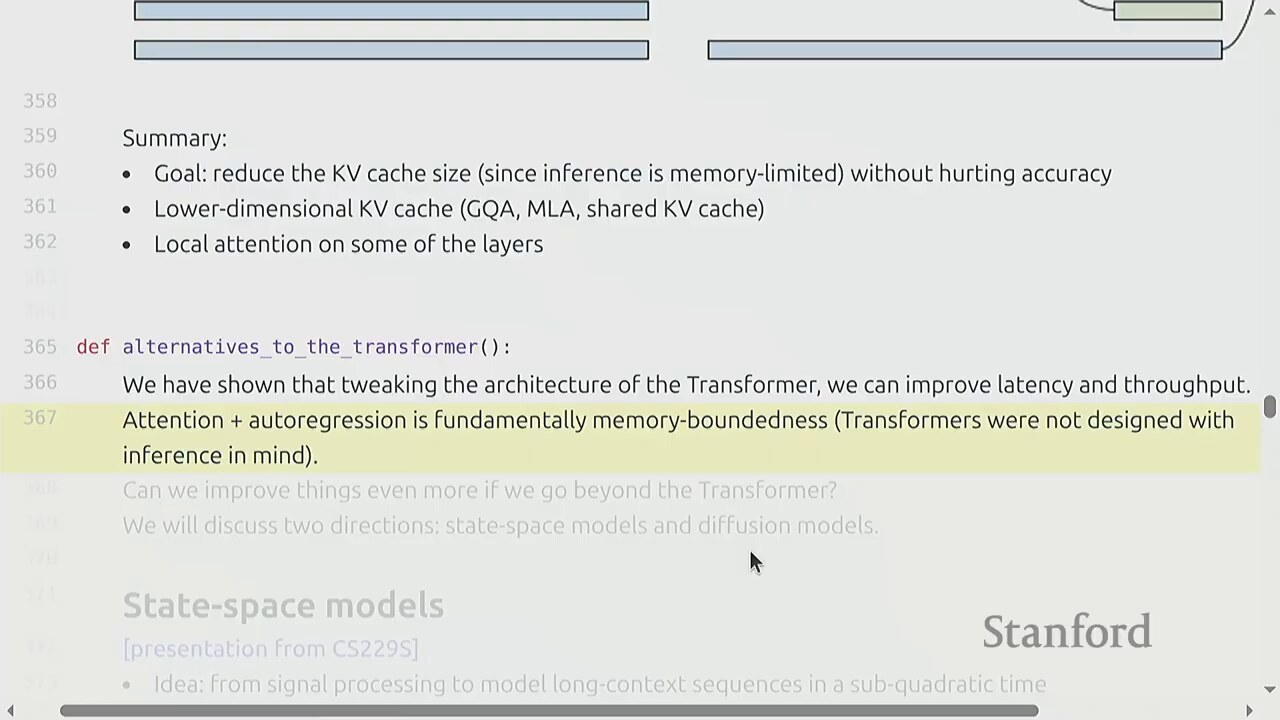
\includegraphics[width=\textwidth]{figures/fig_22_ssm.jpg}
\caption{SSM / Mamba：固定大小隐状态替代变长 KV cache\protect\footnotemark}
\end{figure}
\footnotetext{视频画面时间区间：00:53:15--00:53:45。}

\[
h_t = A \, h_{t-1} + B \, x_t, \qquad y_t = C \, h_t
\]

\begin{itemize}
\item $h_t$：时刻 $t$ 的隐状态（固定维度，不随序列增长）
\item $A, B, C$：状态转移、输入、输出矩阵（可学习的参数）
\item $x_t$：当前 token 的输入特征
\end{itemize}

\begin{importantbox}{SSM 的推理优势}
SSM 的隐状态\textbf{大小恒定}，推理时每步的计算量和显存占用与序列长度无关——从根本上解决了注意力的 $O(N)$ 增长问题。训练时也可以做成线性复杂度（不再 $O(N^2)$）。Mamba 等模型让 SSM 在质量上首次追平 Transformer。
\end{importantbox}

\subsection{线性注意力}

线性注意力是注意力的"软"替代：用核函数 $\phi$ 把 $Q, K, V$ 改写，让复杂度从 $O(N^2)$ 降到 $O(N)$：

\begin{figure}[H]
\centering
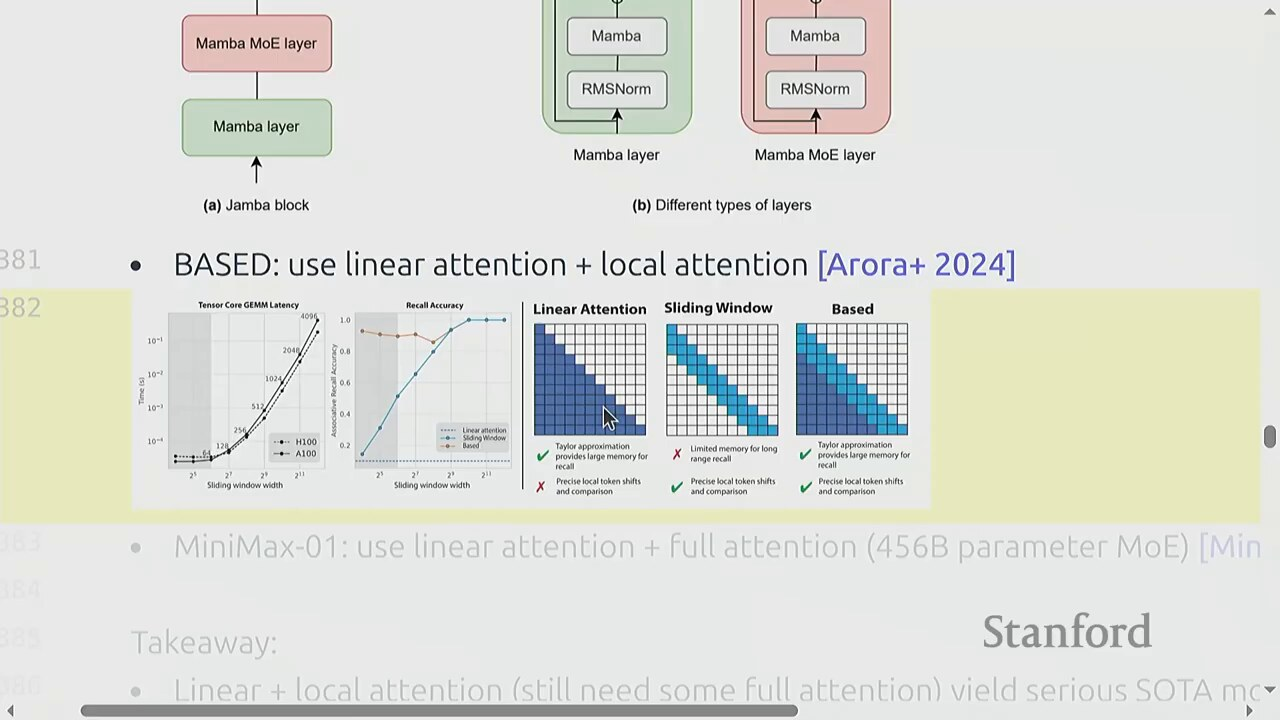
\includegraphics[width=\textwidth]{figures/fig_23_linear.jpg}
\caption{线性注意力：用核函数把 $O(N^2)$ 改写为 $O(N)$\protect\footnotemark}
\end{figure}
\footnotetext{视频画面时间区间：00:58:15--00:58:45。}

\[
\text{Attn}(Q,K,V) = \text{softmax}\!\left(\frac{Q K^\top}{\sqrt{d}}\right) V
\quad\longrightarrow\quad
\phi(Q) \big(\phi(K)^\top V\big)
\]

\begin{itemize}
\item 左式：标准注意力，复杂度 $O(N^2)$（每对 token 都要点积）
\item 右式：线性注意力，先把 $\phi(K)^\top V$ 算成一个固定大小的"记忆矩阵"，再乘 $\phi(Q)$，复杂度 $O(N)$
\item $\phi$：核函数，把 $Q, K$ 映射到某个特征空间（例如 $\phi(x) = \text{elu}(x)+1$）
\end{itemize}

\begin{knowledgebox}{线性注意力的现代复兴}
MiniMax 456B 等新模型大量采用线性注意力变体——大部分层用线性注意力（保持 $O(N)$），只在关键层保留标准注意力（保留表达力）。这种\textbf{混合架构}是当前试图兼得速度和质量的主流方向。
\end{knowledgebox}

\subsection{扩散式语言模型}

最后还提到了一类\textbf{非自回归}的方案——扩散模型（diffusion）。它不再"一个一个 token 往外吐"，而是从噪声出发、\textbf{并行}地去噪出一整段文本：

\begin{figure}[H]
\centering
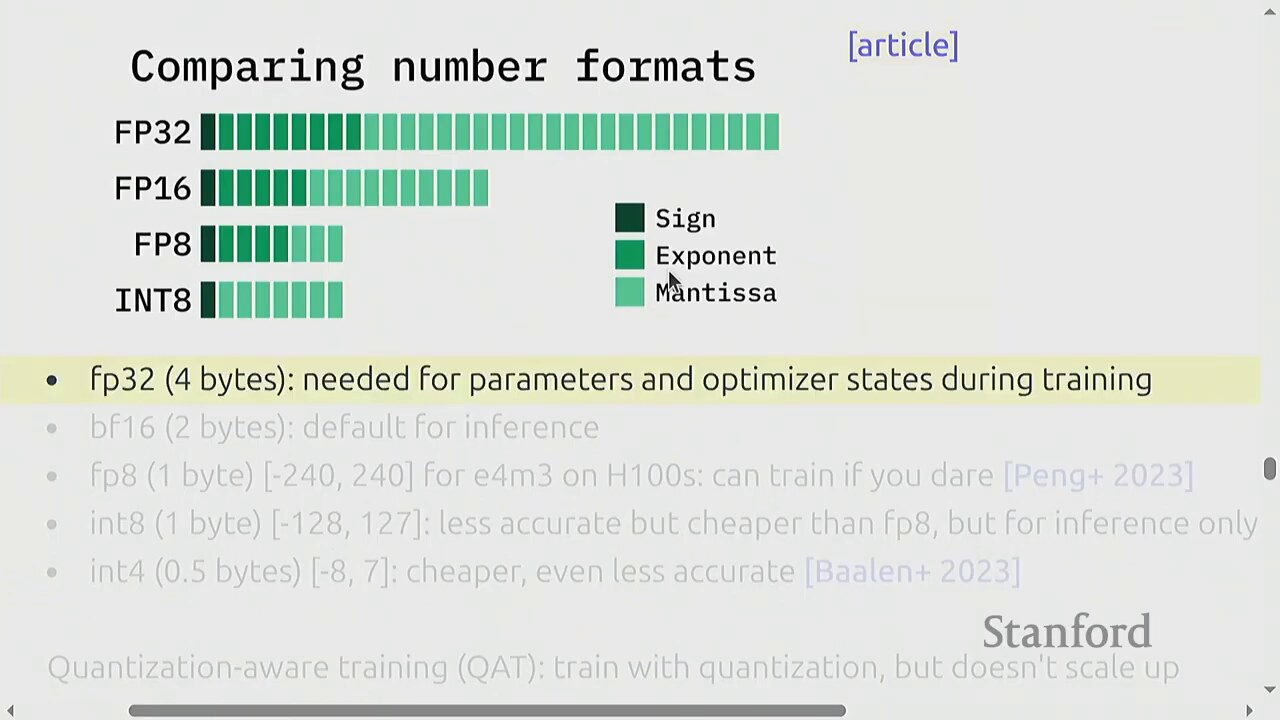
\includegraphics[width=\textwidth]{figures/fig_25_quant.jpg}
\caption{从训练完的模型出发：用更少比特存储权重与激活（量化）\protect\footnotemark}
\end{figure}
\footnotetext{视频画面时间区间：01:05:15--01:05:45。}

\begin{warningbox}{扩散 LLM 的潜力与挑战}
扩散式生成把"自回归的串行"变成"并行的去噪"，理论上吞吐可以大幅提升。Sohl-Dickboy 等的早期工作和近期的图像生成成功给了信心。但语言是离散的，把连续去噪搬到离散 token 上"相当 tricky"，目前质量还没追上自回归。这是一个值得关注的开放方向。
\end{warningbox}

\section{量化：用更少比特存储}

架构改造是"从根上动刀"，\textbf{量化}（quantization）则是"不动架构、只动精度"——用更少的比特来存权重和激活。

\begin{figure}[H]
\centering
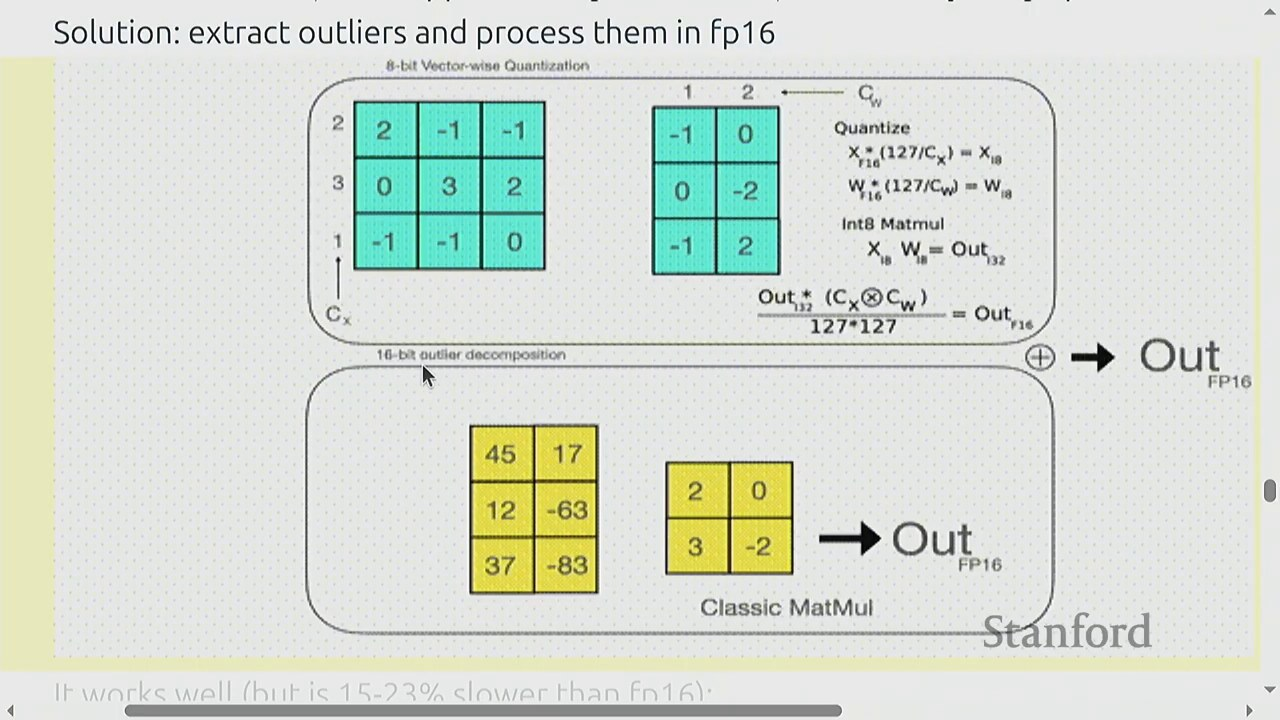
\includegraphics[width=\textwidth]{figures/fig_26_int8.jpg}
\caption{INT8 量化：把 BF16 权重压成 8 比特\protect\footnotemark}
\end{figure}
\footnotetext{视频画面时间区间：01:07:45--01:08:15。}

BF16 是推理的默认精度（每个数 16 比特）。量化就是把它压成 INT8（8 比特）、甚至 INT4（4 比特）：

\[
x_{\text{int8}} = \text{round}\!\left(\frac{x}{s}\right), \qquad s = \frac{\max|x|}{127}
\]

\begin{itemize}
\item $x$：原始 BF16 权重值
\item $s$：缩放因子，由权重的最大绝对值决定
\item $x_{\text{int8}}$：量化后的 8 比特整数（$-128$ 到 $127$）
\end{itemize}

\begin{importantbox}{量化的两倍收益}
权重从 16 比特降到 8 比特：（1）显存占用减半；（2）带宽受限的解码阶段，每秒能读的\textbf{权重数翻倍}，吞吐直接翻倍。降到 4 比特就是 4 倍。这是性价比极高的优化。
\end{importantbox}

\subsection{INT8 的麻烦：异常值}

但 INT8 不是白吃的午餐。问题在于：权重的分布\textbf{不均匀}，有些通道的值远大于其他——这些\textbf{异常值}（outliers）会迫使缩放因子 $s$ 变大，结果让其他正常值被量化到只剩几个离散档位，精度严重损失。

\begin{warningbox}{LLM.int8() 的发现}
Tim Dettmers 等人发现：LLM 里极少数通道（可能 $< 0.1\%$）的激活值异常大，却携带了关键信息。把它们和大多数正常值一起做 INT8，等于把整批数据"按最坏情况"压缩。LLM.int8() 的解法是：\textbf{把异常值挑出来单独用 BF16 算，其余做 INT8}——保住了关键信息又拿到大部分加速。
\end{warningbox}

\subsection{AWQ：激活感知的权重量化}

\textbf{Activation-aware Weight Quantization}（AWQ）走另一条路：不是看权重大小，而是看\textbf{哪些权重对激活更敏感}。对应大激活的通道，保留更高精度；其他激进压到 4 比特。

\subsection{蒸馏与剪枝：从大模型蒸馏到小模型}

除了降精度，还可以\textbf{直接换一个更小的模型}：

\begin{figure}[H]
\centering
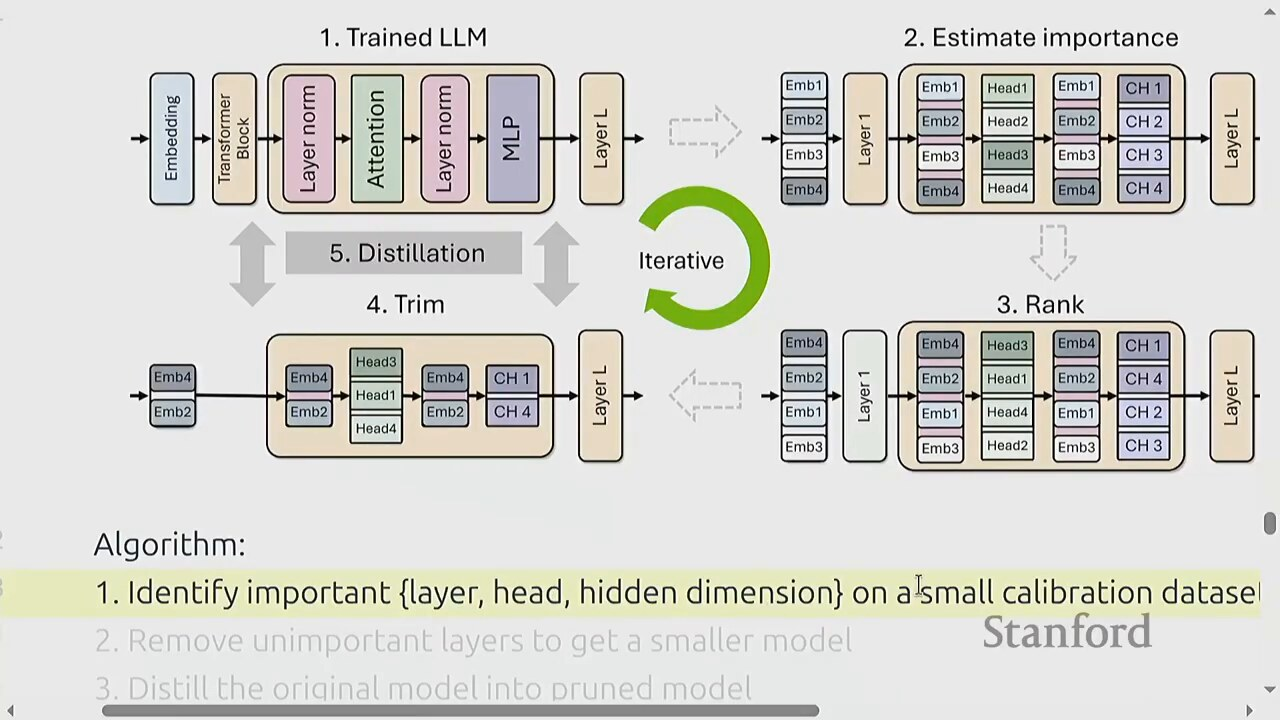
\includegraphics[width=\textwidth]{figures/fig_27_distill.jpg}
\caption{蒸馏：用大模型（教师）的输出训练小模型（学生）\protect\footnotemark}
\end{figure}
\footnotetext{视频画面时间区间：01:09:15--01:09:45。}

\begin{tabular}{p{3cm}p{11cm}}
\toprule
\textbf{方法} & \textbf{核心思想} \\
\midrule
剪枝（pruning） & 把不重要的权重置零（结构化剪枝删整个通道），减少计算 \\
蒸馏（distillation） & 用大模型（教师）的 logits 或中间特征当监督，训练一个更小的学生模型 \\
\bottomrule
\end{tabular}

\begin{knowledgebox}{为什么这些都是"lossy"}
量化、剪枝、蒸馏都是\textbf{有损}（lossy）的——它们用一点点质量换取大幅的速度或显存收益。关键问题永远是："这点质量损失能不能用更多训练或更聪明的算法补回来？"GPT-4、Llama 系列都是 4 比特推理，说明行业已经接受了这个权衡。
\end{knowledgebox}

\section{投机解码：用小模型猜，大模型验}

到目前为止的所有优化都没改一个事实：每个 token 都要让大模型算一遍。\textbf{投机解码}（speculative decoding）打破这个限制——让一个\textbf{小的草稿模型}（draft model）先猜好几个 token，大模型再一次性验证：

\begin{figure}[H]
\centering
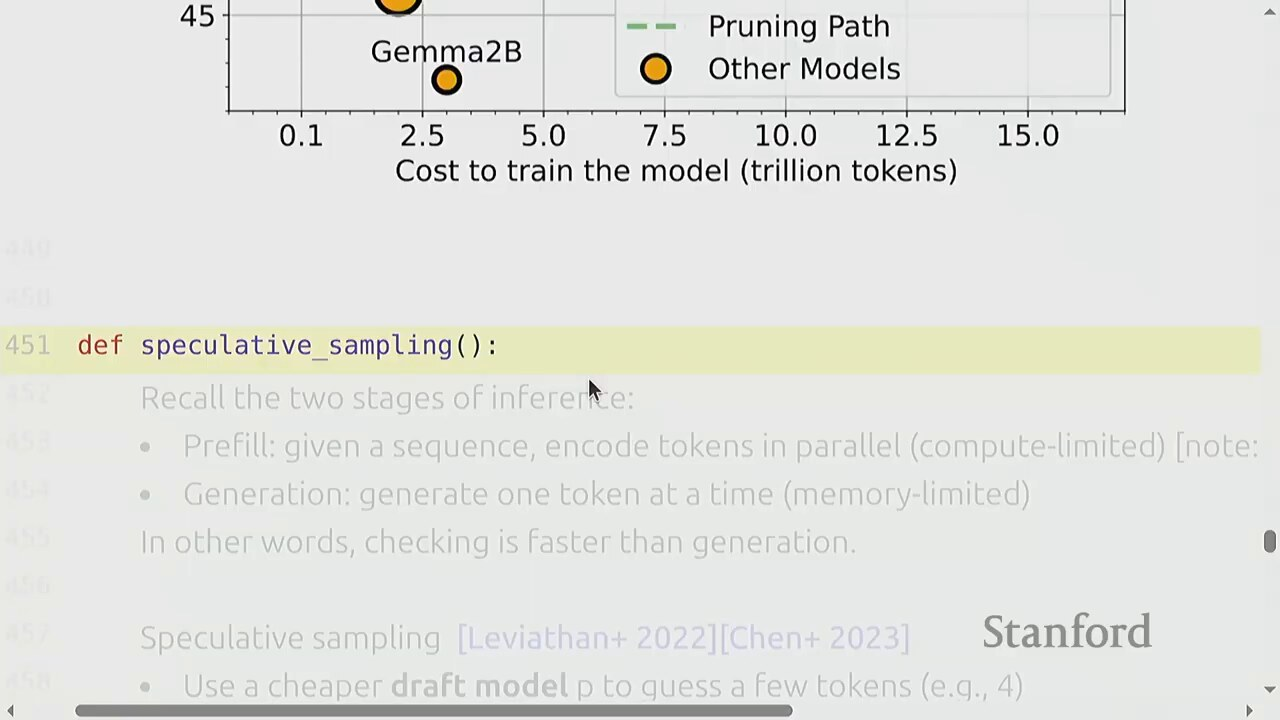
\includegraphics[width=\textwidth]{figures/fig_28_spec.jpg}
\caption{投机解码：草稿模型快速生成 $\gamma$ 个候选 token，目标模型一次验证\protect\footnotemark}
\end{figure}
\footnotetext{视频画面时间区间：01:11:15--01:11:45。}

\subsection{流程：草稿 + 验证}

\begin{enumerate}
\item 草稿模型（小、快）自回归生成 $\gamma$ 个候选 token：$x_1, x_2, \dots, x_\gamma$
\item 目标模型（大、准）\textbf{一次性}把这 $\gamma$ 个 token 当输入做一次前向，得到每个位置的概率 $q_t$（目标分布）
\item 对比草稿模型的概率 $p_t$ 和目标的 $q_t$，决定接受哪些 token
\end{enumerate}

\begin{importantbox}{为什么这是算力的胜利}
解码阶段大模型是带宽受限、算力闲置的。投机解码让大模型\textbf{一次前向同时验证多个 token}——多读几个 token 几乎不增加带宽压力（反正权重都得读），却把闲置的算力用上了。只要草稿模型猜得准，吞吐就能翻倍。
\end{importantbox}

\subsection{拒绝采样：保证分布完全一致}

最妙的是，投机解码可以用\textbf{拒绝采样}（rejection sampling）严格保证：最终输出的分布\textbf{和直接用大模型采样完全一样}。没有任何质量损失：

\begin{figure}[H]
\centering
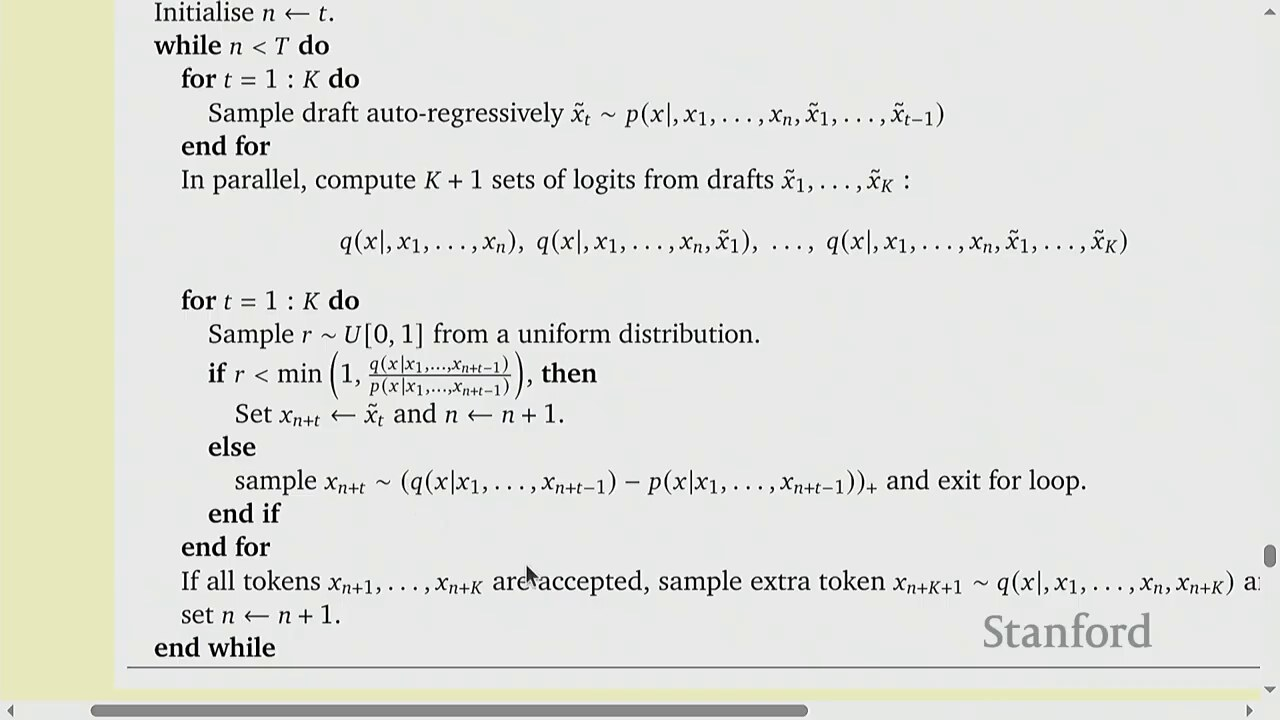
\includegraphics[width=\textwidth]{figures/fig_29_reject.jpg}
\caption{投机解码 = 用 $P$（草稿）做提案的拒绝采样，保证最终分布与 $Q$（目标）完全一致\protect\footnotemark}
\end{figure}
\footnotetext{视频画面时间区间：01:14:15--01:14:45。}

对草稿模型给出的 token $x$（草稿概率 $p(x)$，目标概率 $q(x)$）：

\[
\text{接受概率} = \min\!\left(1, \frac{q(x)}{p(x)}\right)
\]

\begin{itemize}
\item $p(x)$：草稿模型给出 token $x$ 的概率
\item $q(x)$：目标模型给 token $x$ 的概率
\item 若 $q(x) \ge p(x)$：草稿低估了这个 token，直接接受（接受概率 1）
\item 若 $q(x) < p(x)$：草稿高估了，按 $q(x)/p(x)$ 的概率接受；若拒绝，按 $(q - p)^+$ 重采样
\end{itemize}

\begin{knowledgebox}{拒绝采样的数学保证}
可以严格证明：经过上述接受/拒绝后，最终输出 token 的分布就是 $q$。\textbf{投机解码不是近似}——它产出的序列和"大模型直接采样"在统计上完全等价。这是一个"既快又准"的稀有案例，理论保证了质量无损。
\end{knowledgebox}

\subsection{实证：约 2 倍加速}

实测中，配一个 70 亿参数的草稿模型给 700 亿的目标模型，通常能拿到\textbf{约 2 倍}的吞吐提升——因为草稿模型猜得相当准，大部分 token 都被接受，大模型每步确实能"白拿"好几个 token。

\begin{practicebox}{草稿模型的选择}
草稿模型不必和目标模型同族——只要分布够接近就行。研究热点包括：用更小的同架构模型、用知识蒸馏专门训一个"模仿者"、甚至用模型前面几层当草稿（layer-skipping）。关键权衡：草稿模型越准，接受率越高，但生成越慢；越快，每秒提议越多，但接受率越低。
\end{practicebox}

\section{服务层优化：批处理与内存管理}

最后 Percy 转向\textbf{serving 系统}层面——即便模型和架构都不变，调度策略也能大幅提升吞吐。

\subsection{连续批处理}

朴素的批处理（static batching）要等凑齐一批再一起发，发完再凑下一批。问题是请求长度不一——长请求拖累整批，短请求空等：

\begin{figure}[H]
\centering
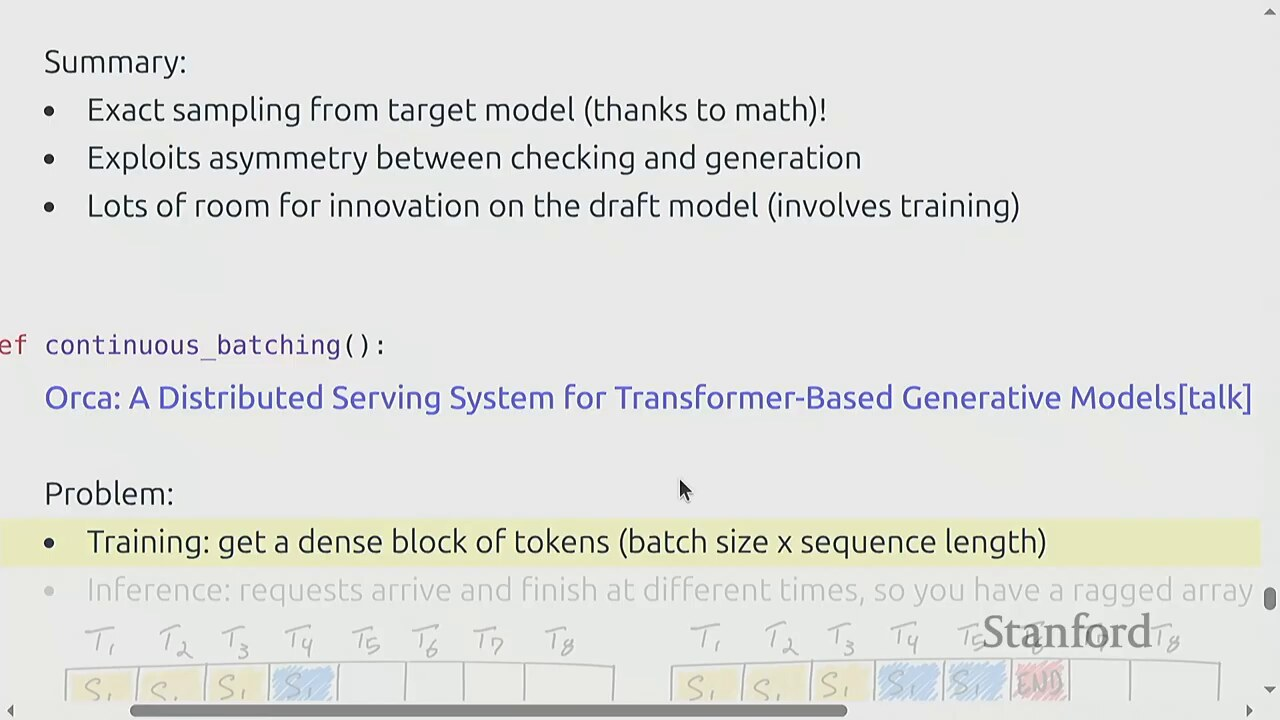
\includegraphics[width=\textwidth]{figures/fig_30_contbatch.jpg}
\caption{连续批处理：请求级动态进出，不等整批\protect\footnotemark}
\end{figure}
\footnotetext{视频画面时间区间：01:17:45--01:18:15。}

\begin{importantbox}{连续批处理的核心}
连续批处理（continuous batching，又称 iteration-level batching）在\textbf{每个解码步}都重新组批：新请求随时加入、完成的请求随时退出。不再等整批——GPU 始终在满批量运转。这是 vLLM、TGI 等现代推理框架的标配。
\end{importantbox}

\subsection{PagedAttention：KV cache 的虚拟内存}

连续批处理有个难题：每个请求的 KV cache 长度不同、还在动态变化，传统的"连续分配一大块"会导致严重的\textbf{显存碎片}——很多空隙用不上。vLLM 的 \textbf{PagedAttention} 借鉴操作系统的\textbf{虚拟内存}思想解决它：

\begin{figure}[H]
\centering
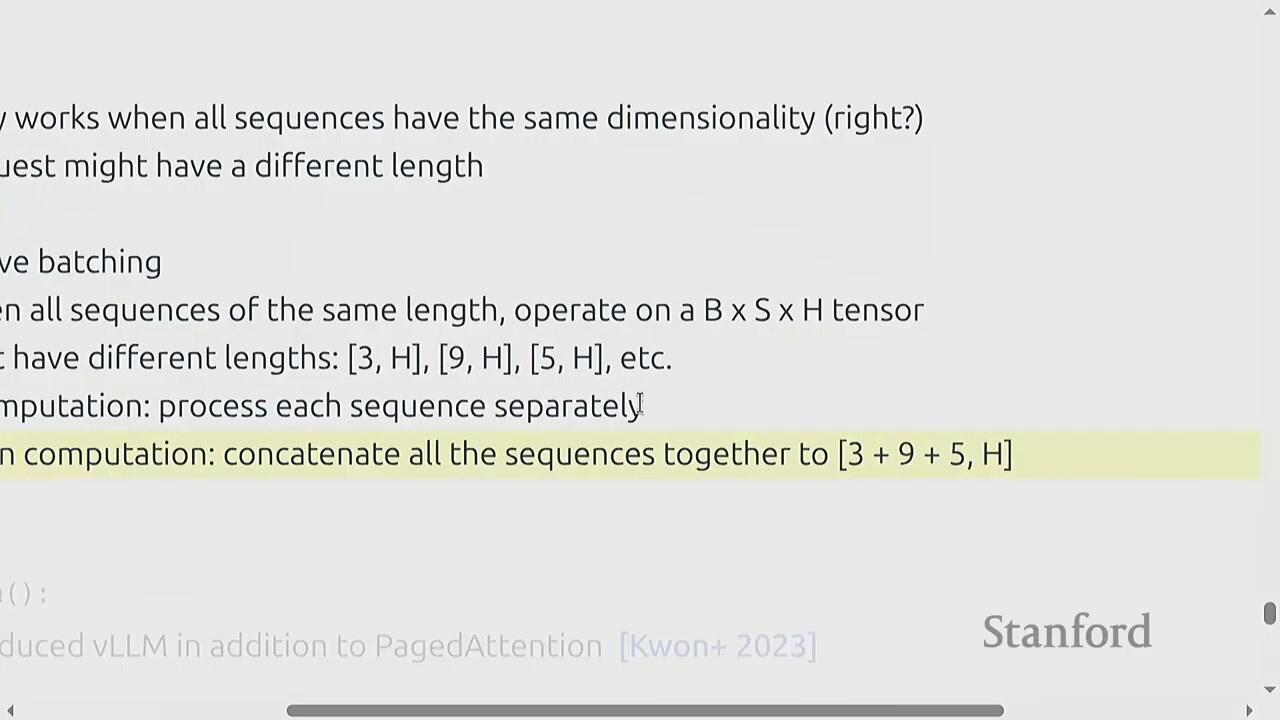
\includegraphics[width=\textwidth]{figures/fig_31_paged.jpg}
\caption{PagedAttention：KV cache 拆成固定大小的"页"，按需分配\protect\footnotemark}
\end{figure}
\footnotetext{视频画面时间区间：01:19:15--01:19:45。}

把每个请求的 KV cache 拆成固定大小的\textbf{块}（block），通过一个\textbf{页表}（block table）映射到物理显存。请求增长时按需申请新块，结束时整块释放。

\begin{tabular}{p{3.5cm}p{3cm}p{7.5cm}}
\toprule
\textbf{类比} & \textbf{操作系统} & \textbf{PagedAttention} \\
\midrule
虚拟地址空间 & 进程的虚拟内存 & 一个请求逻辑上的连续 KV cache \\
物理内存 & 物理内存页 & GPU 上固定大小的 KV block \\
映射 & 页表 & block table \\
碎片问题 & 外部碎片 & 请求间显存碎片 \\
\bottomrule
\end{tabular}

\begin{knowledgebox}{PagedAttention 的三大收益}
（1）\textbf{消除外部碎片}：块可以放在显存任何空位，利用率接近 100\%；（2）\textbf{支持变长请求}：请求增长时按需申请新块，不用预留；（3）\textbf{支持共享}：多个请求共享同一个前缀（如系统 prompt）的 KV 块。
\end{knowledgebox}

\subsection{写时复制：共享前缀}

当很多请求共用同一段前缀（例如同一个 system prompt），没必要每个请求都存一份这段 KV。PagedAttention 用\textbf{写时复制}（copy-on-write）让它们指向同一组物理块：

\begin{figure}[H]
\centering
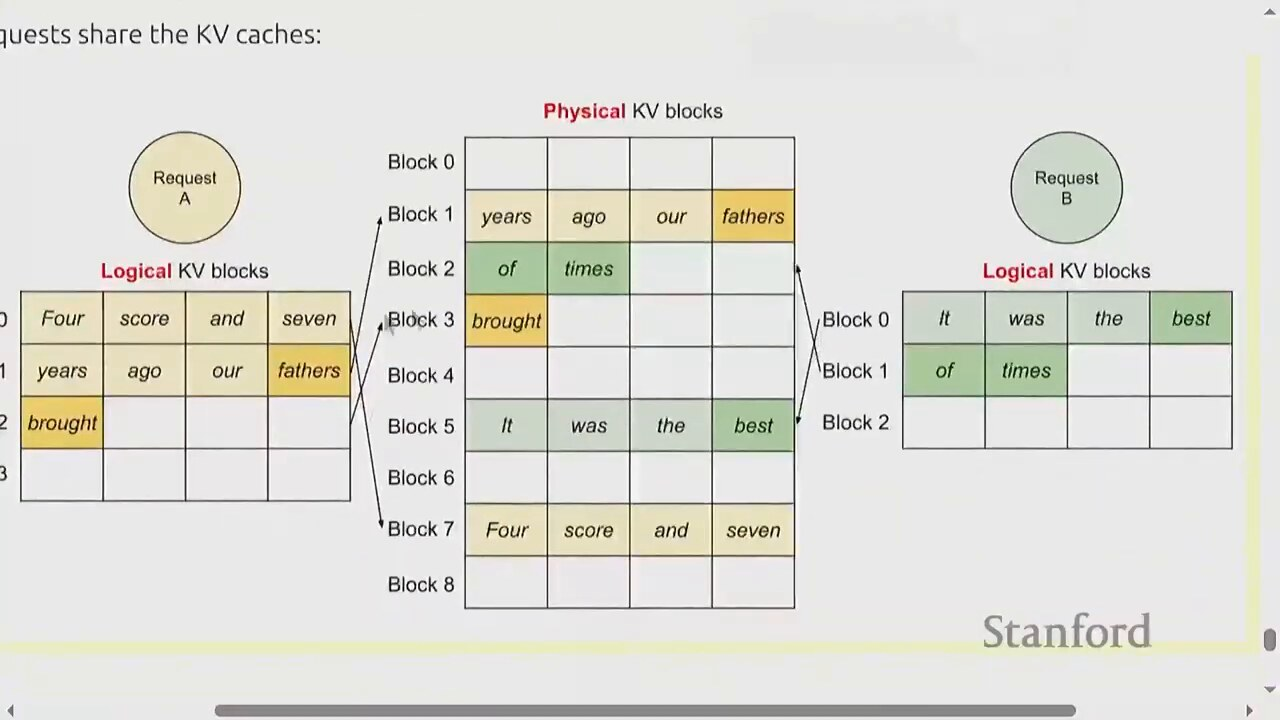
\includegraphics[width=\textwidth]{figures/fig_32_cow.jpg}
\caption{写时复制：共享前缀的 KV 块，只在分歧时复制\protect\footnotemark}
\end{figure}
\footnotetext{视频画面时间区间：00:20:15--00:20:45。}

\begin{itemize}
\item 维护每个块的\textbf{引用计数}（reference count），记录有多少请求在用它
\item 引用计数 $>1$ 的块是只读共享的
\item 只有当某个请求要"分叉"出自己的 KV 时，才复制那一个块（写时复制）
\end{itemize}

\begin{importantbox}{共享前缀的实战价值}
在 agent、RAG、多轮对话场景，大量请求共享同一段长 system prompt 或长文档。共享前缀能把这段 KV 的显存和计算成本\textbf{摊薄到所有请求}——这是现代 LLM serving 的一个巨大效率来源。
\end{importantbox}

\section{总结与延伸}

\subsection{算术强度：贯穿全讲的统一线索}

\begin{figure}[H]
\centering
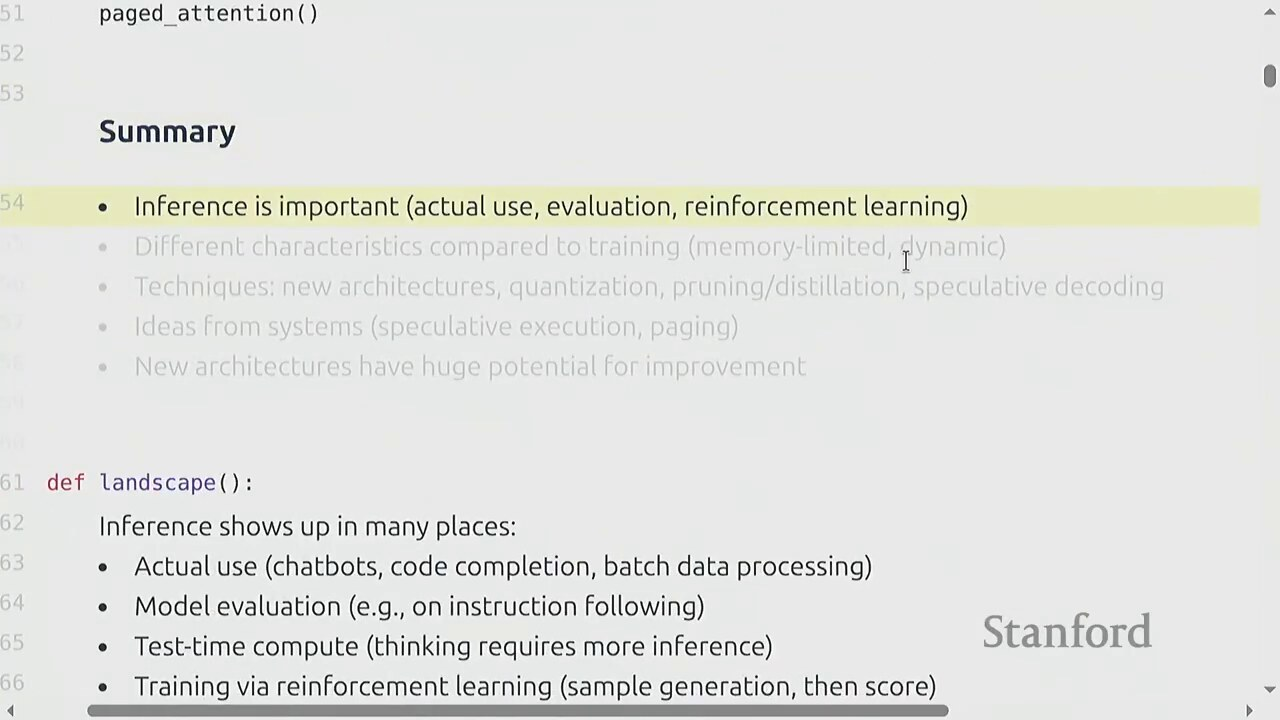
\includegraphics[width=\textwidth]{figures/fig_33_concl.jpg}
\caption{总结：算术强度框架把所有推理优化技术串成一条线\protect\footnotemark}
\end{figure}
\footnotetext{视频画面时间区间：01:21:15--01:21:45。}

\begin{importantbox}{六个核心论点}
\begin{enumerate}
\item \textbf{算术强度是推理优化的罗盘}：每个算子的 $I$ 与 GPU 阈值 $I^*$ 比较，立刻知道是算力受限还是带宽受限。所有优化都在围绕"提高 $I$"或"省带宽"。
\item \textbf{推理分两阶段、瓶颈不同}：Prefill 是 compute-bound（吃算力），Decode 是 memory-bound（吃带宽）。两阶段的优化策略完全不同。
\item \textbf{$B=1$ 是带宽地狱}：单请求解码算术强度 $\approx 1$，GPU 算力利用率不到 1/300。批量是第一救命稻草。
\item \textbf{KV cache 是显存天花板}：随序列线性增长，是批量大小的硬限制。GQA/MLA/SSM 都在攻击它。
\item \textbf{量化是性价比之王}：4 比特推理在工业界已是标配，吞吐直接翻几倍，质量损失可接受。
\item \textbf{投机解码是稀有的"无损加速"}：用拒绝采样保证分布不变，实测 2 倍提速。理论保证 + 工程收益，这是最佳实践。
\end{enumerate}
\end{importantbox}

\subsection{技术地图回顾}

\begin{tabular}{p{4cm}p{4cm}p{6cm}}
\toprule
\textbf{优化方向} & \textbf{代表技术} & \textbf{攻击的瓶颈} \\
\midrule
改架构 & GQA, MLA, CLA, 局部注意力 & KV cache 体积 \\
换范式 & SSM/Mamba, 线性注意力, 扩散 LLM & $O(N^2)$ 或 $O(N)$ 增长 \\
降精度 & INT8/INT4, LLM.int8(), AWQ & 带宽、显存 \\
压缩模型 & 剪枝、蒸馏 & 算力、显存 \\
算法层 & 投机解码 & 闲置算力（带宽受限时） \\
服务层 & 连续批处理, PagedAttention, 共享前缀 & 碎片、空转、冗余存储 \\
\bottomrule
\end{tabular}

\subsection{下节预告}

后续讲座会进一步讨论\textbf{训练系统的并行策略}（数据并行、张量并行、流水线并行、FSDP）以及\textbf{长上下文}与\textbf{MoE}（混合专家）架构——它们既是训练的关键技术，也深刻影响推理时的成本结构。

\subsection{配套阅读}

以下论文/系统建议按本讲主题阅读：

\begin{tabular}{p{7cm}p{6cm}}
\toprule
\textbf{论文/系统} & \textbf{对应知识点} \\
\midrule
GQA (Ainslie 2023) & Grouped-Query Attention \\
DeepSeek-V2/V3 技术报告 & MLA 多头潜在注意力 \\
Mamba (Gu \& Dao 2023) & 状态空间模型 \\
vLLM (Kwon 2023) & PagedAttention, 连续批处理 \\
Speculative Decoding (Leviathan 2023) & 投机解码 + 拒绝采样 \\
LLM.int8() (Dettmers 2022) & 异常值感知的 INT8 量化 \\
AWQ (Lin 2023) & 激活感知权重量化 \\
FlashAttention (Dao 2022) & IO 感知的精确注意力 \\
\bottomrule
\end{tabular}

%% --- 正文内容结束 ---

\end{document}
